\chapter{Discrete cosine transform} \label{DCT}
A discrete cosine transform (DCT) expresses a finite sequence of data points in terms of a sum of cosine functions oscillating at different frequencies. DCTs are important to numerous applications in science and engineering, from lossy compression of audio (e.g. MP3) and images (e.g. JPEG).
The DCT is often used in signal and image processing, especially for lossy compression, because it has a strong "energy compaction" property: in typical applications, most of the signal information tends to be concentrated in a few low-frequency components of the DCT.

There are different variations of the discrete cosine transform, but the most common one is the "DCT-II" which is also used in JPEG image compression and by MATLAB \circledR:



  \begin{equation} \label{eq:dct_eq}	
   X_{k}= \sum_{n=0}^{N-1} w(k)x_{n}cos\bigg[\frac{\pi}{N} (n+\frac{1}{2})k\bigg], \qquad k=0,1,...,N-1
 \end{equation}
 

    \[
    w(x)=\left\{
    \begin{array}{ll}
    \frac{1}{\sqrt{N}} & \qquad k=0\\
    &\\
    \sqrt{\frac{2}{N}} & \qquad 1\leqslant k \leqslant N-1\\
    \end{array}
    \right.
    \]
\bigskip
We can see the equation \ref{eq:dct_eq} as a product of matrices: we have to multiply the input vector $ x_{i} $  with a matrix of coefficients for cosine.
Thus the equation \ref{eq:dct_eq} can be rewritten as 

\begin{center}
\bigskip	
$\begin{bmatrix}X_{0}\\ X_{1} \\ \vdots \\X_{N-1} \end{bmatrix} = 
\begin{bmatrix}
	cos_{0,0} & cos_{0,1} & \cdots & cos_{0,n-1} \\
	cos_{1,0} & cos_{1,1} & \cdots & cos_{1,n-1} \\
	\vdots  & \vdots  & \ddots & \vdots  \\
	cos_{n-1,0} & cos_{n-1,1} & \cdots & cos_{n-1,n-1}  \\
\end{bmatrix} \begin{bmatrix}x_{0}\\ x_{1} \\ \vdots \\x_{N-1} \end{bmatrix}$

\end{center}
\bigskip
where the matrix of coefficients for cosine is the following

\begin{center}	
$ \begin{bmatrix} \frac{1}{\sqrt{N}}cos(\frac{\pi}{N}(0+\frac{1}{2})\cdotp 0) & \frac{1}{\sqrt{N}}cos(\frac{\pi}{N}(1+\frac{1}{2})\cdotp 0) & \cdots & \frac{1}{\sqrt{N}}cos(\frac{\pi}{N}(N-1+\frac{1}{2})\cdotp 0) \\
\sqrt{\frac{2}{N}}cos(\frac{\pi}{N}(0+\frac{1}{2})\cdotp 1) & \sqrt{\frac{2}{N}}cos(\frac{\pi}{N}(1+\frac{1}{2})\cdotp 1) & \cdots & \sqrt{\frac{2}{N}}cos(\frac{\pi}{N}(N-1+\frac{1}{2})\cdotp 1) \\
\vdots  & \vdots  & \ddots & \vdots  \\
\sqrt{\frac{2}{N}}cos(\frac{\pi}{N}(0+\frac{1}{2})\cdotp N-1) & \sqrt{\frac{2}{N}}cos(\frac{\pi}{N}(1+\frac{1}{2})\cdotp N-1) & \cdots & \sqrt{\frac{2}{N}}cos(\frac{\pi}{N}(N-1+\frac{1}{2})\cdotp N-1) \end{bmatrix} $
\bigskip
\end{center}

  \section{Hardware Implementation} \label{DCTH}
The result can be seen as a sum of products.
Each element of the output array can be written as:
\begin{center}
	$ X_{i} =  x_{0}cos_{i,0}+x_{1}cos_{i,1}+ \cdots +x_{n-1}cos_{i,n-1}$
\end{center}

Therefore, since there is no data dependencies between these elemnts, we can evaluate them in parallel.
\begin{enumerate}
\item In the first clock cycle we can perform the multiplication $ x_{0}cos_{i,0} $ for each element of the array.
\item In the second clock cycle we evaluate the second multiplication and sum it to the previous result $  [x_{0}cos_{i,0}] + x_{1}cos_{i,1} $
\item In the third clock cycle we evaluate the third multiplication and sum it to the previous result $  [x_{0}cos_{i,0} + x_{1}cos_{i,1}] + x_{2}cos_{i,2}$
\item We repeat this process until we reach the last term of this sum of product. In this clock cycle we have the final result $ X_{i} =  x_{0}cos_{i,0}+x_{1}cos_{i,1}+ \cdots +x_{n-1}cos_{i,n-1}  $

\end{enumerate}

In the following, we have the process explained in a matrix form, while figure \ref{fig:dct_scheme} represents this implementation in a Register to Transfer Level.


\begin{center}
	\bigskip	
	$\begin{bmatrix}X_{0}\\ X_{1} \\ \vdots \\X_{N-1} \end{bmatrix} = 
	\begin{bmatrix}
	
	\begin{matrix}
		x_{0}cos_{0,0}\\
		x_{0}cos_{1,0}\\
		\vdots\\
		\underbrace{x_{0}cos_{n-1,0}}_{1^{st} step}
		
		\end{matrix}
		
		\begin{matrix}
		\quad+\quad\\
		\quad+\quad\\
		\quad	\vdots\\
		\quad+\quad\\
		\\
		\end{matrix}
		
	\begin{matrix}
	x_{1}cos_{0,1}\\
	x_{1}cos_{1,1}\\
	\vdots\\
	\underbrace{x_{1}cos_{n-1,1}}_{2^{nd} step}
	
	\end{matrix}
	
		\begin{matrix}
		\quad+\quad\\
		\quad+\quad\\
		\quad\vdots\\
		\quad+\quad\\
		\\
		\end{matrix}
	
	\begin{matrix}
	\quad\cdots\\
	\quad\cdots\\
	\quad\vdots\\
	\quad\cdots\\
	\\
	\end{matrix}
	
		\begin{matrix}
		\quad+\quad\\
		\quad+\quad\\
		\quad\vdots\\
		\quad+\quad\\
		\\
		\end{matrix}
		
		\begin{matrix}
		x_{n-1}cos_{0,n-1}\\
		x_{n-1}cos_{1,n-1}\\
		\vdots\\
		\underbrace{x_{n-1}cos_{n-1,n-1}}_{last \quad step}
		
		\end{matrix}

	\end{bmatrix} $
	
\end{center}
\bigskip
\begin{figure}[h!]
	\centering	
	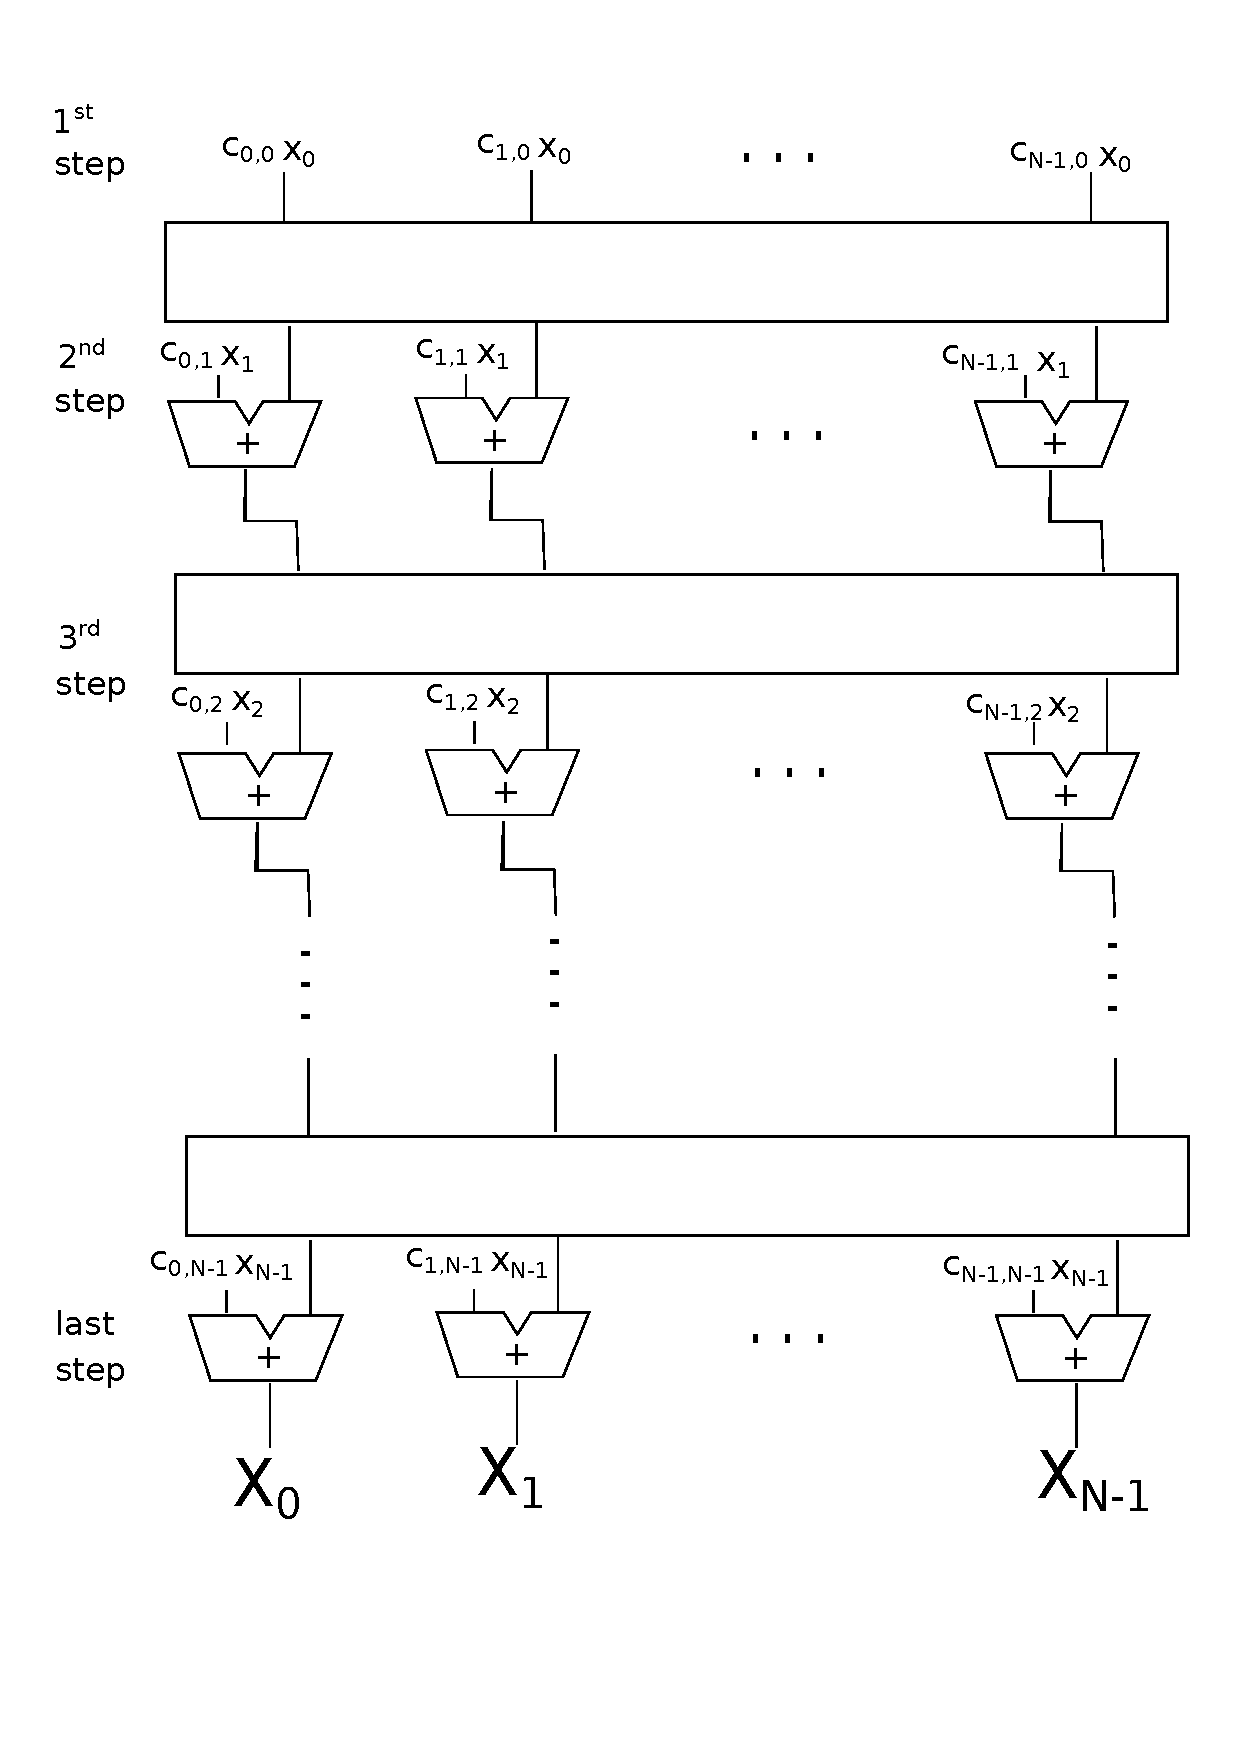
\includegraphics[width=0.9\textwidth]{imm/dct/dct_scheme.pdf}  
	\caption{Implementation of DCT algorithm} 
	\label{fig:dct_scheme}
\end{figure}
\clearpage
\section{Simulation and Test} 
I performed some tests of this implementation with different size and dimension. In the fig.\ref{fig:tb_dct} we can see the results of an array of six elements.

\begin{figure}[h!]
	\centering	
	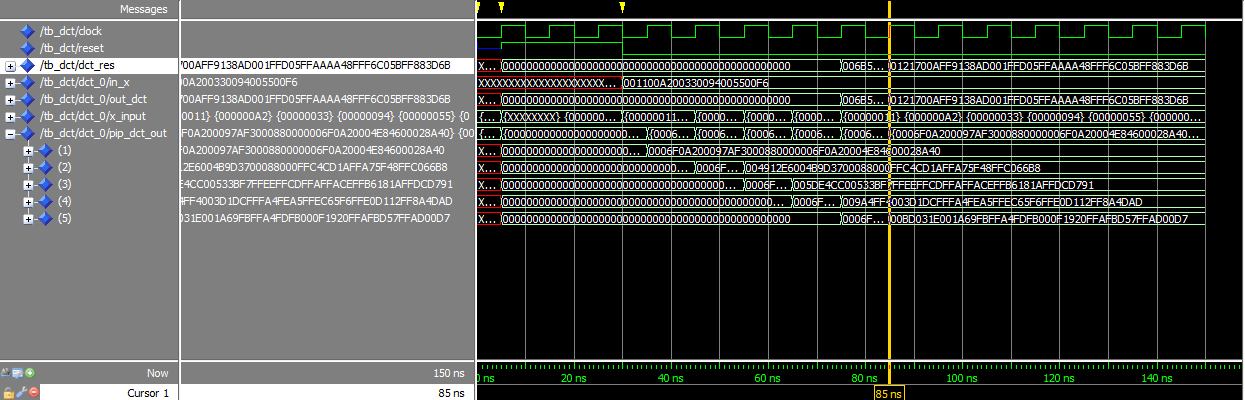
\includegraphics[width=\textwidth]{imm/dct/wave1.png}  
	\caption{Discrete cosine transform-Results of the simulation} 
	\label{fig:tb_dct}
\end{figure}
The simulation shows the input array:
\begin{center}
	$ in\_x=0x001100A200330094005500F6$ 
\end{center}
that stands for 
\begin{center}
	$ x_{0}=0x0011$\\
$ 	x_{1}=0x00A2 $\\
	$ x_{2}=0x0033 $ \\
	$ x_{3}=0x0094 $ \\
	$ x_{4}=0x0055 $ \\
	$x_{5}=0x00F6$
\end{center} which in decimal is
\begin{center}

$ x_{0}=17$ \\$ x_{1}=162 $\\$ x_{2}=51 $\\$ x_{3}=148 $\\$ x_{4}=85 $\\$x_{5}=246$
\end{center}
During the first 6 clock cycles, we can see the partial sum and multiplications.
The output is available in the $ 6^{th} $ clock cycle after the reset:\begin{center}
	 $ dct\_res=0x0121700AFF9138AD001FFD05FFAAAA48FFF6C05BFF883D6B $
\end{center} that stands for\begin{center}
 $ X_{0}=0x0121700A$ \\$X_{1}=0xFF9138AD$\\$X_{2}=0x001FFD05$\\$X_{3}=0xFFAAAA48
 $\\$X_{4}=0xFFF6C05B$\\$X_{5}=0xFF883D6B $
\end{center} and if we convert them in decimal by reserving 16 bits for the floating points, we get 
\begin{center}
	 $ X_{0}=289.437653$\\$X_{1}=-110.778610$\\$X_{2}=31.988358$\\$X_{3}=-85.334839$
	 \\$X_{4}=-9.248611$\\$X_{5}=-119.760086 $
\end{center}
 We checked this result by using the function $ dct $ on Matlab (Figure \ref{fig:dct_res_mat}).
We see that it differs from the Matlab result by a value in the order of 1/100. This depends on the precision used for the implementation, especially when converting the cosine values into binary.
 




\begin{figure}[h!]
	\centering	
	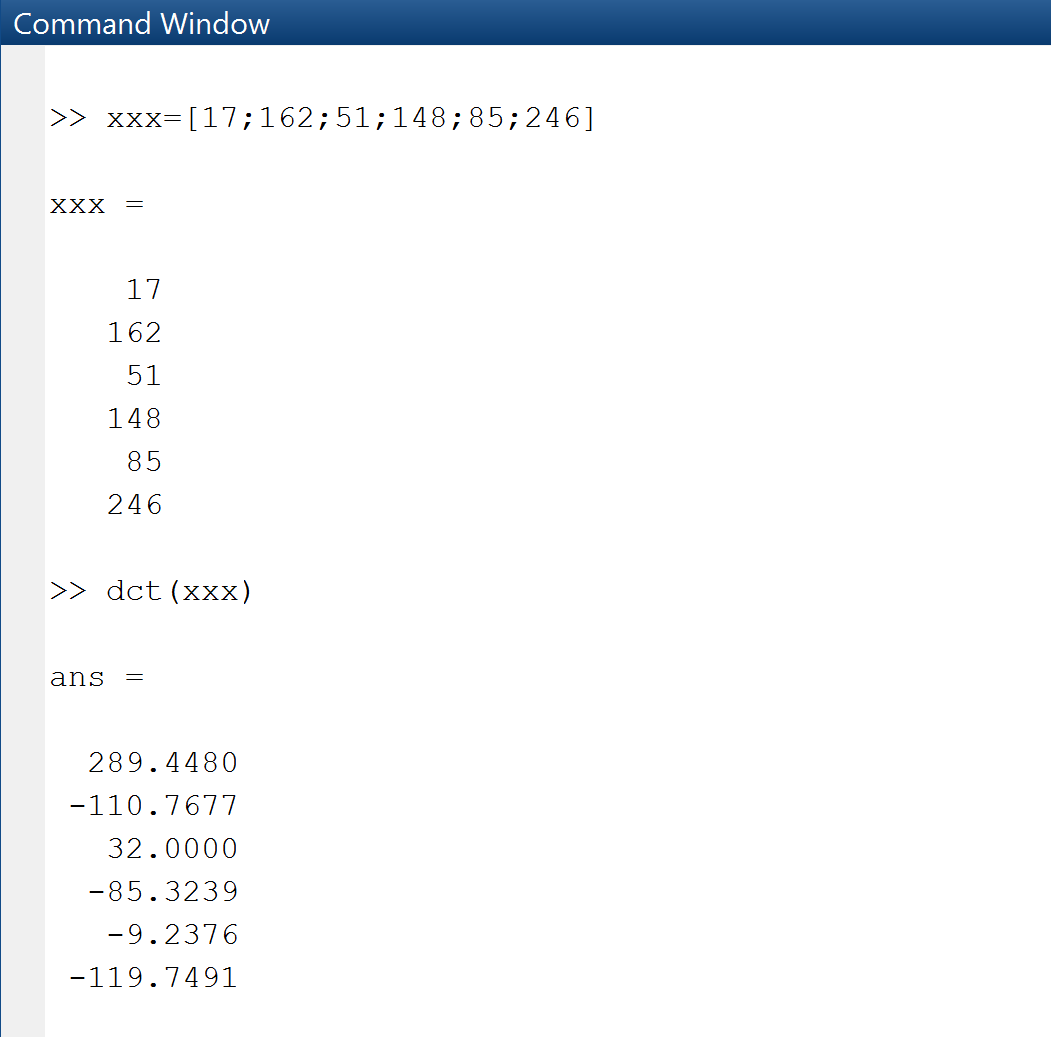
\includegraphics[width=0.9\textwidth]{imm/dct/dct_res_matlab.png}  
	\caption{DCT result in MATLAB} 
	\label{fig:dct_res_mat}
\end{figure}

\clearpage
\section{Comparison}
 \subsection{Systolic array architecture}
A systolic array can be seen as a homogeneous network of funtional units (called also \textbf{nodes} or \textit{Data Processing Units (DPU)}) which elaborate data and exchange them with their neighbours following a flow; in particular each FU receives the data from its upstream FU, elaborates it and passes it downstream. 
Each FU is indipendent from the others and executes only one operation over a huge amount of data; for this reason, systolic arrays are classified as SIMD (single instruction, multiple data) architectures. 
The particular name ("systolic") derives from the fact that inside the array there is a continuous flow of data propagating from a FU to the next one resembling the flow of the blood in the human body.
Usually, systolic arrays cannot be programmed and for this reason the circuit has to be designed $ ad-hoc $. This kind of structure is made of simple FUs which usually implement a simple operation (addition, multiplication, ecc..) and that have a very small memory capability. The main purpose of each node is to compute a data and send it to the next FU following the flow. 

\begin{figure}[h!]
	\centering	
	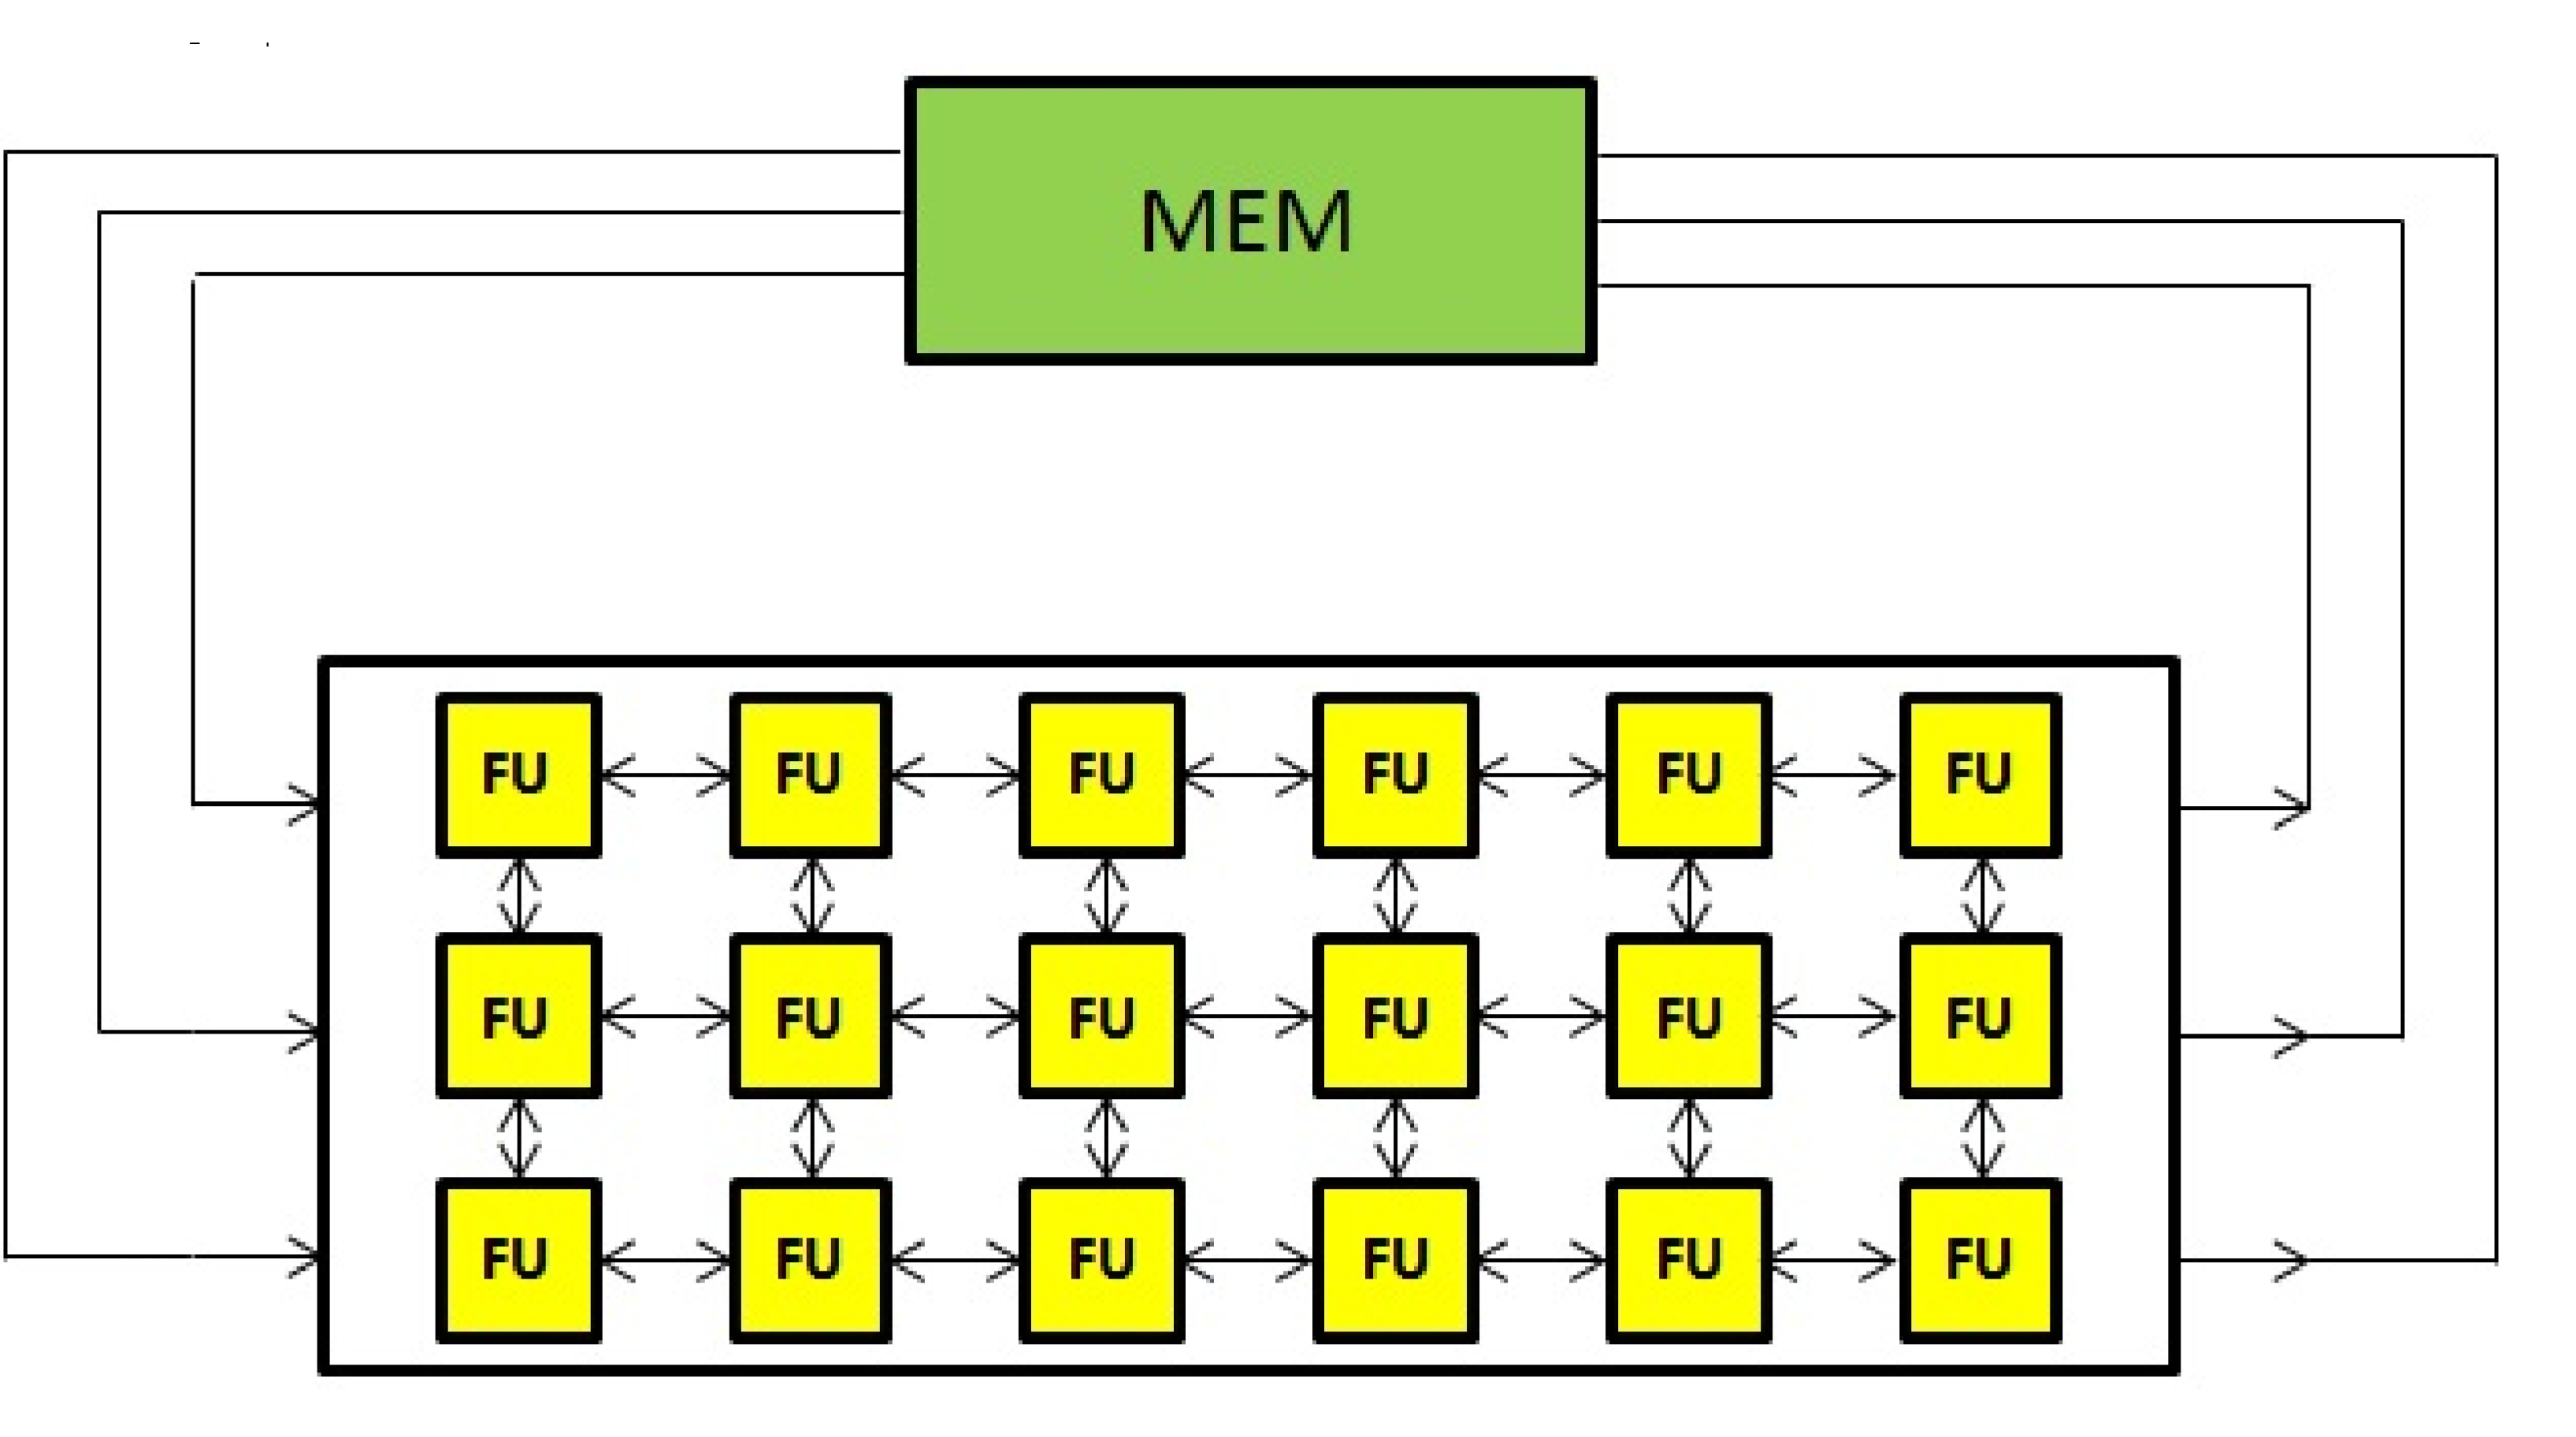
\includegraphics[width=0.9\textwidth]{imm/dct/dct_sa0.png}  
	\caption{ A generic figure of a systolic array; it is possible to notice the presence of parallel inputs and parallel outputs. Data are taken from the memory, eleborated along the multiple paths of FUs and then stored again in the memory.
		} 
	\label{fig:dct_sa0}
\end{figure}
\clearpage
 \subsection{Comparison with systolic array implementation}  \label{DCTSA}
 The DCT has been implemented in a systolic array architecture with the following structure (Fig \ref{fig:dct_sa1})
 
 \begin{figure}[h!]
 	\centering
 	 	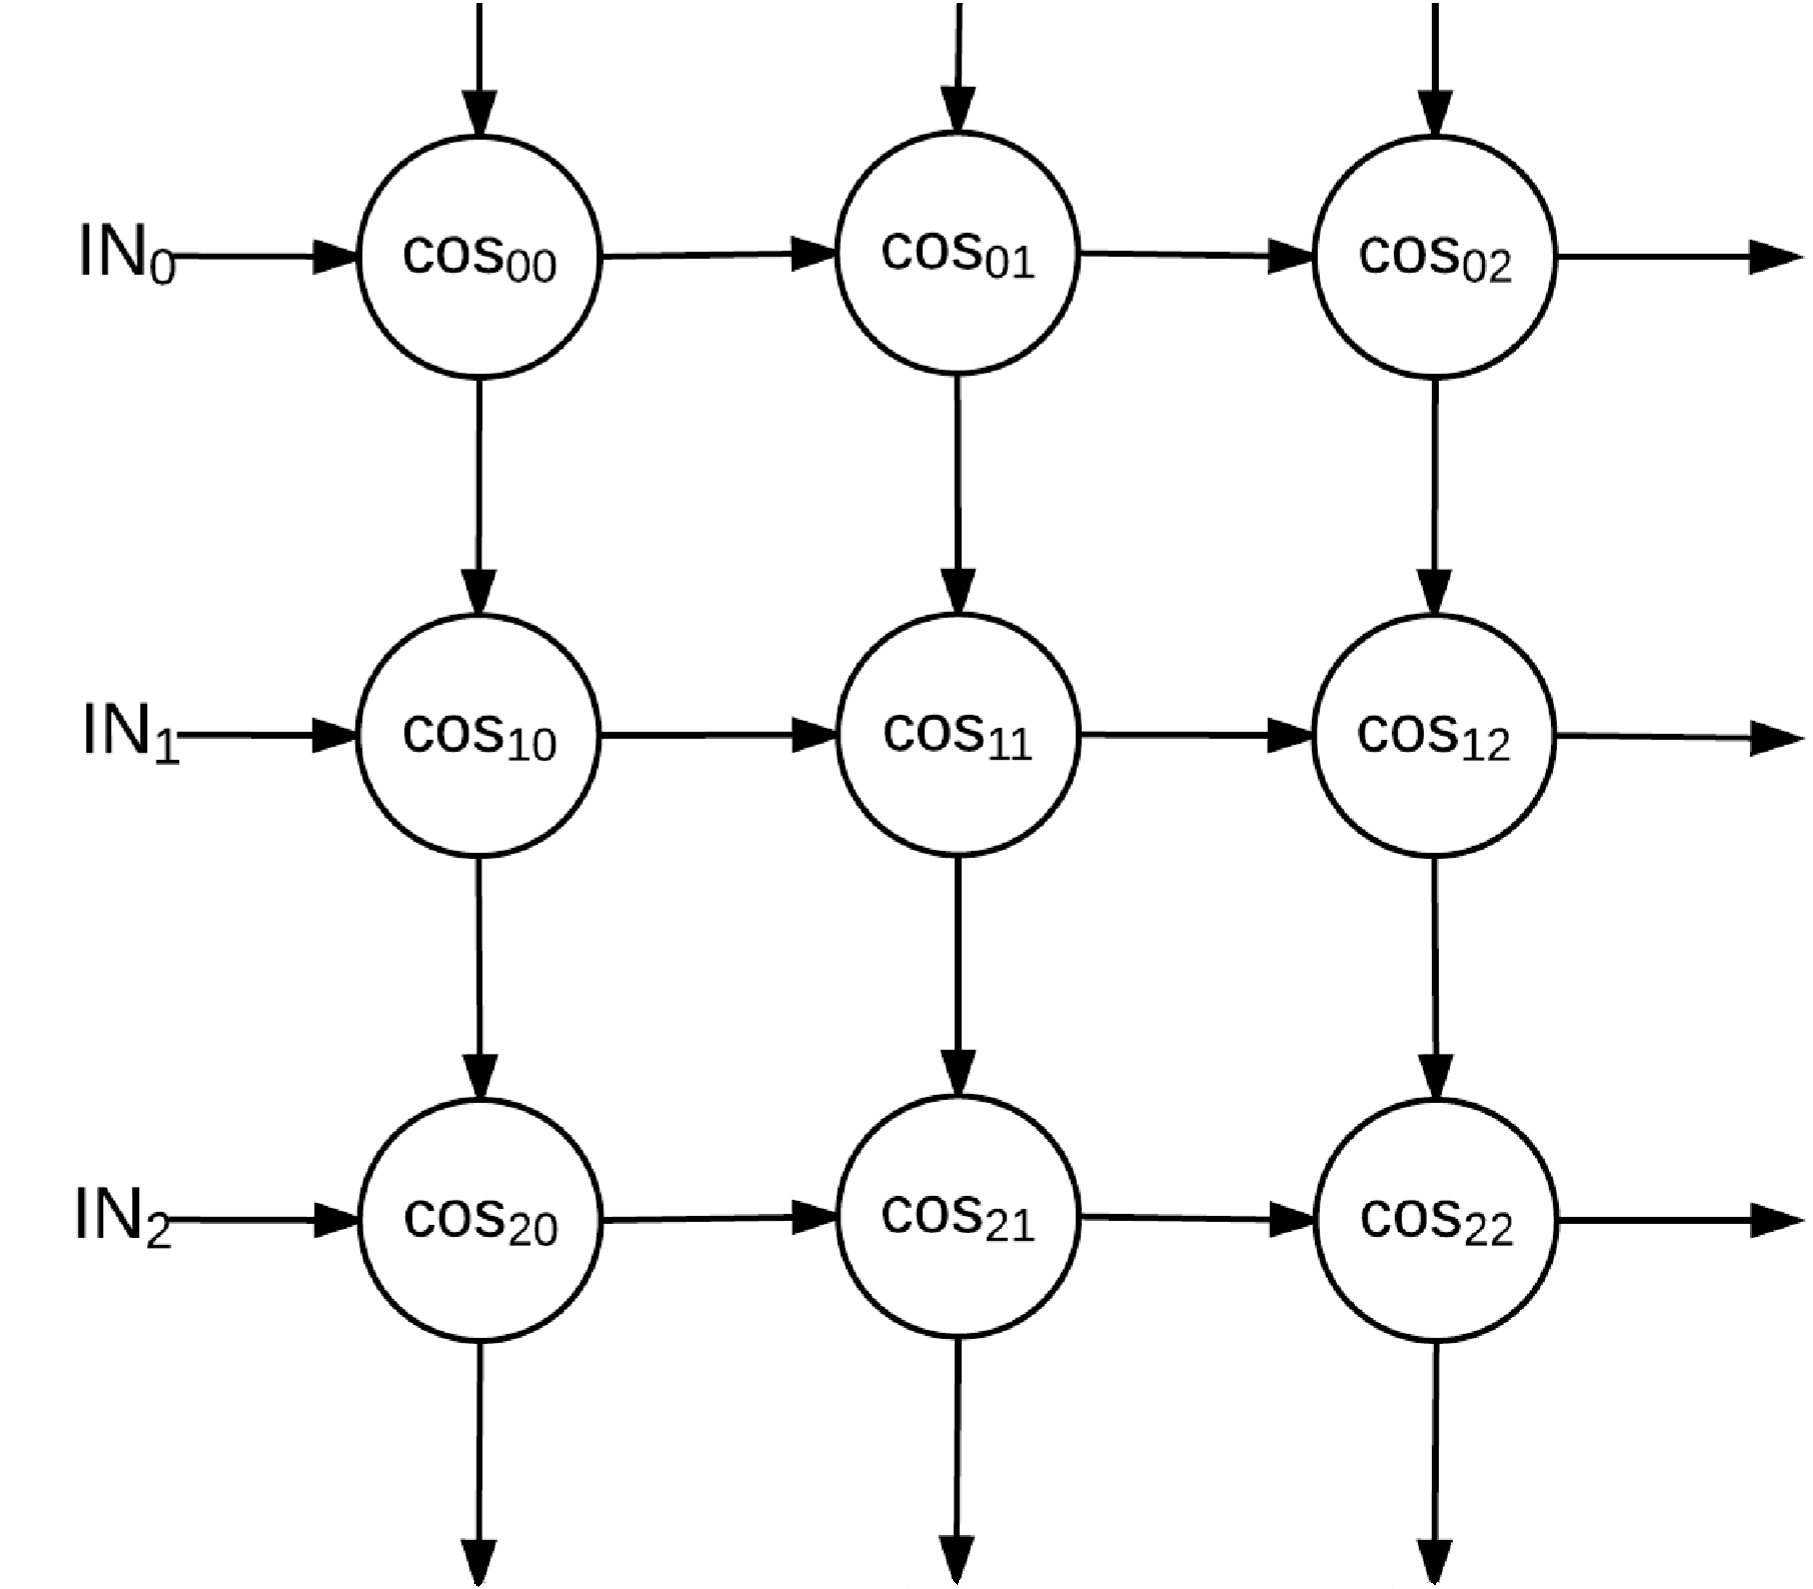
\includegraphics[width=0.75\textwidth]{imm/dct/dct_sa1.png}  
 	% 	\resizebox{[width=\textwidth]}{!}{\input{imm/dct/dct_scheme.pdf_tex}}
 	\caption{Implementation of DCT algorithm in a systolic array architecture} 
 	\label{fig:dct_sa1}
 \end{figure}
 
 Given an input array (from the left), each element of this array will be multiplied by the values of the cosine matrix, previously stored in the internal register (Fig \ref{fig:dct_sa2}).
 At the output of each processing element (Fig \ref{fig:dct_sa2}), we have tha product $ IN_{i}\cdot cos_{i,j} $ towards the bottom and the $ IN_{i} $ value toward the right.
 
  \begin{figure}[h!]
  	\centering
  	  	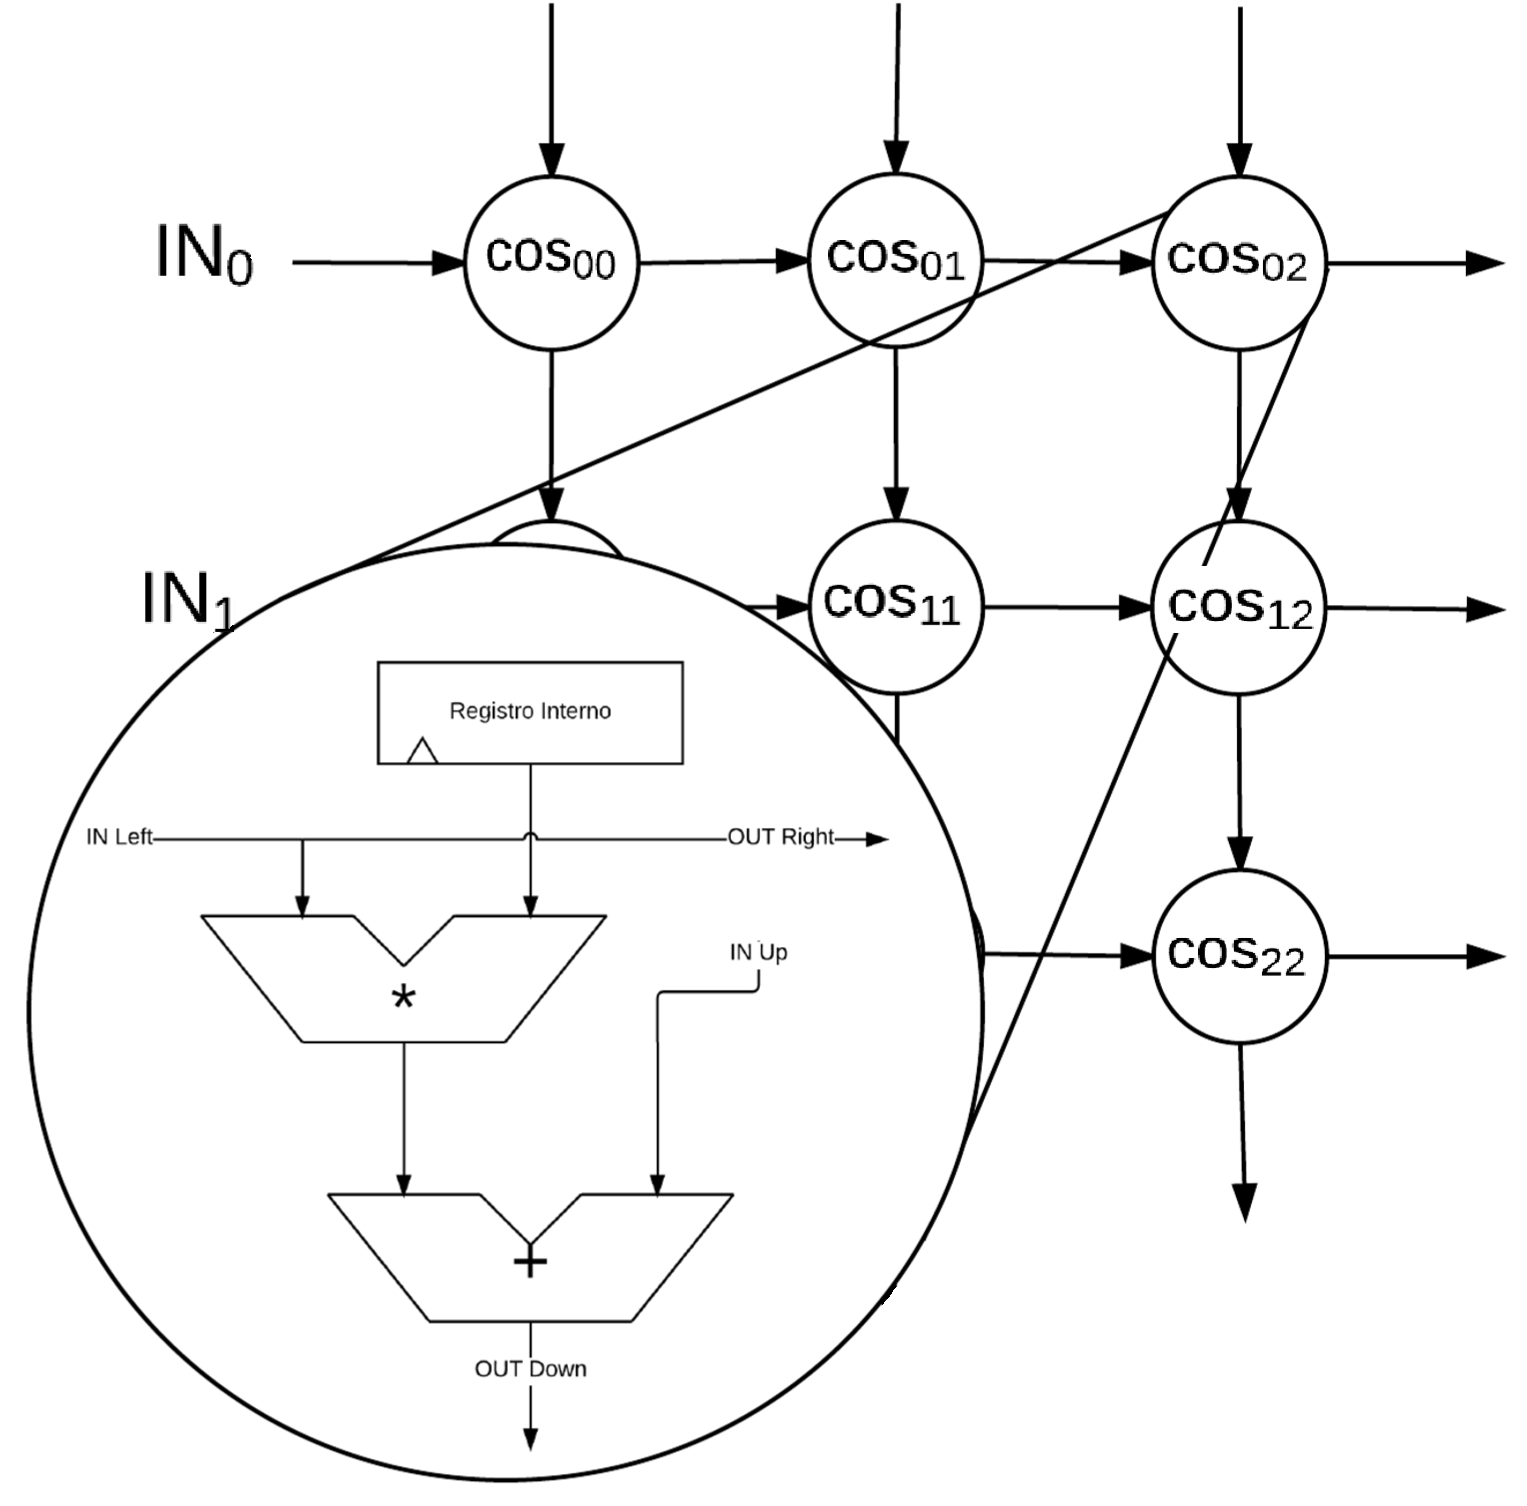
\includegraphics[width=0.75\textwidth]{imm/dct/dct_sa2.png}  
  	% 	\resizebox{[width=\textwidth]}{!}{\input{imm/dct/dct_scheme.pdf_tex}}
  	\caption{Processing element structure} 
  	\label{fig:dct_sa2}
  \end{figure}
   
  The simulation's results of this implementation are shown in figure \ref{fig:dct_sa3} with a check of the result in MATLAB (Fig. \ref{fig:dct_sa4})
  As we can see from the simulation, for an array of size $ N $, we need $ 2N-1 $ clock cycles to get the result.
  On the other hand, by looking to the structure of the systolic array, we can deduct the area to be $ N \cdot N $ processing elements.\\
  An important observation has to be done for the table \ref{table:dct_tab}.
  For the implementation not pipelined described in \ref{DCTH}, the critical path is made of one multiplier and a cascade of $ N-1 $ adders, this is due because all the multiplication can be done in parallel, while the adders have some dependencies between them.
   \begin{center}
   	\begin{tabular}{ | p{1.3cm} | >{\centering\arraybackslash}p{4cm} | >{\centering\arraybackslash}p{4cm} | >{\centering\arraybackslash}p{4cm} |}
   		\hline
   		\label{table:dct_tab} & Systolic array & This work & This work pipelined\\
   		\hline
   		Area & $ N^{2}$ $ moltiplications $ \qquad \qquad$N^{2}$ $ additions $  & $N^{2}
   $ $moltiplications$ \qquad \qquad $ N^{2} $ $additions$ & $ N$ $ moltiplications$ \qquad \qquad $ N$ $ additions$\\
   		\hline
   		Time & $ (2N-1) $ x (time for an addition and a multiplication)&
   		
   		$ (N-1) $x(time for an addition) + time for a single multiplication & time for an addition and a multiplication. Also the synthesy's results \ref{synDCT} are concordant with this theory.
   		 \\
   		\hline
   		
   	\end{tabular}
   \end{center}
        \begin{figure}[h!]
        	\centering
        	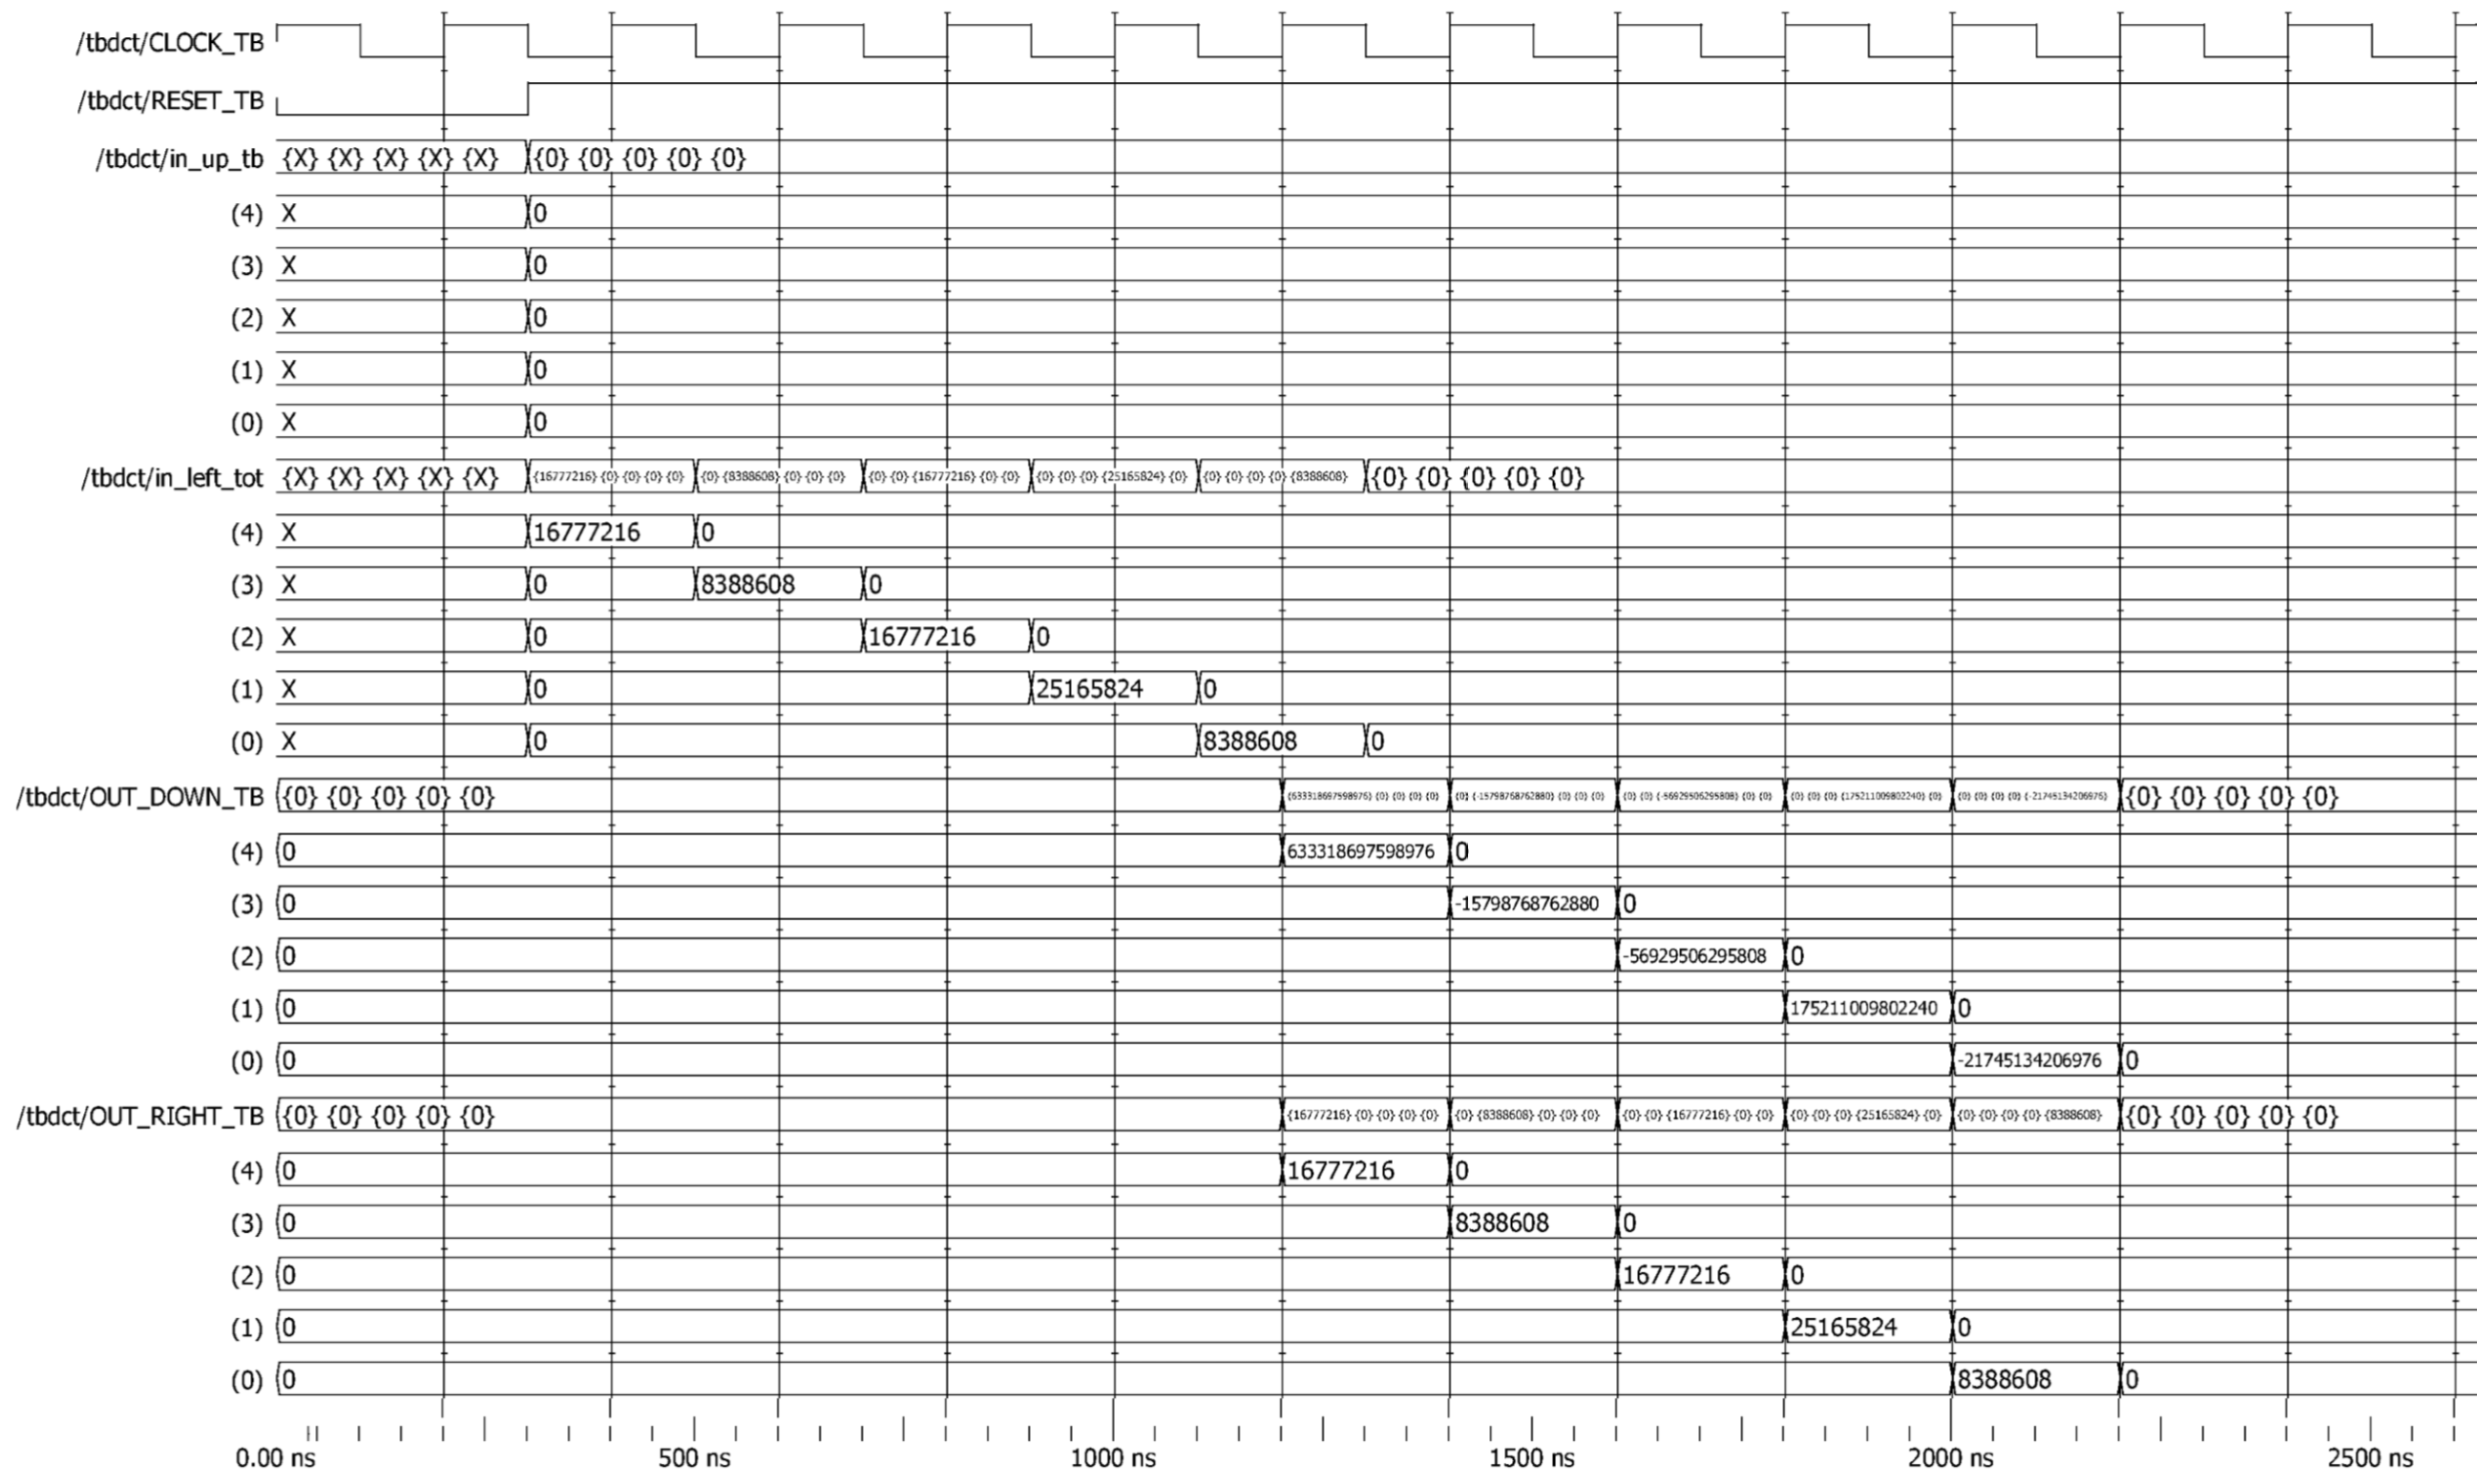
\includegraphics[width=\textwidth]{imm/dct/dct_sa3.png}  
        	\caption{Results of the DCT in a systolic array architecture} 
        	\label{fig:dct_sa3}
        \end{figure}
        
        \begin{figure}[h!]
        	\centering
        	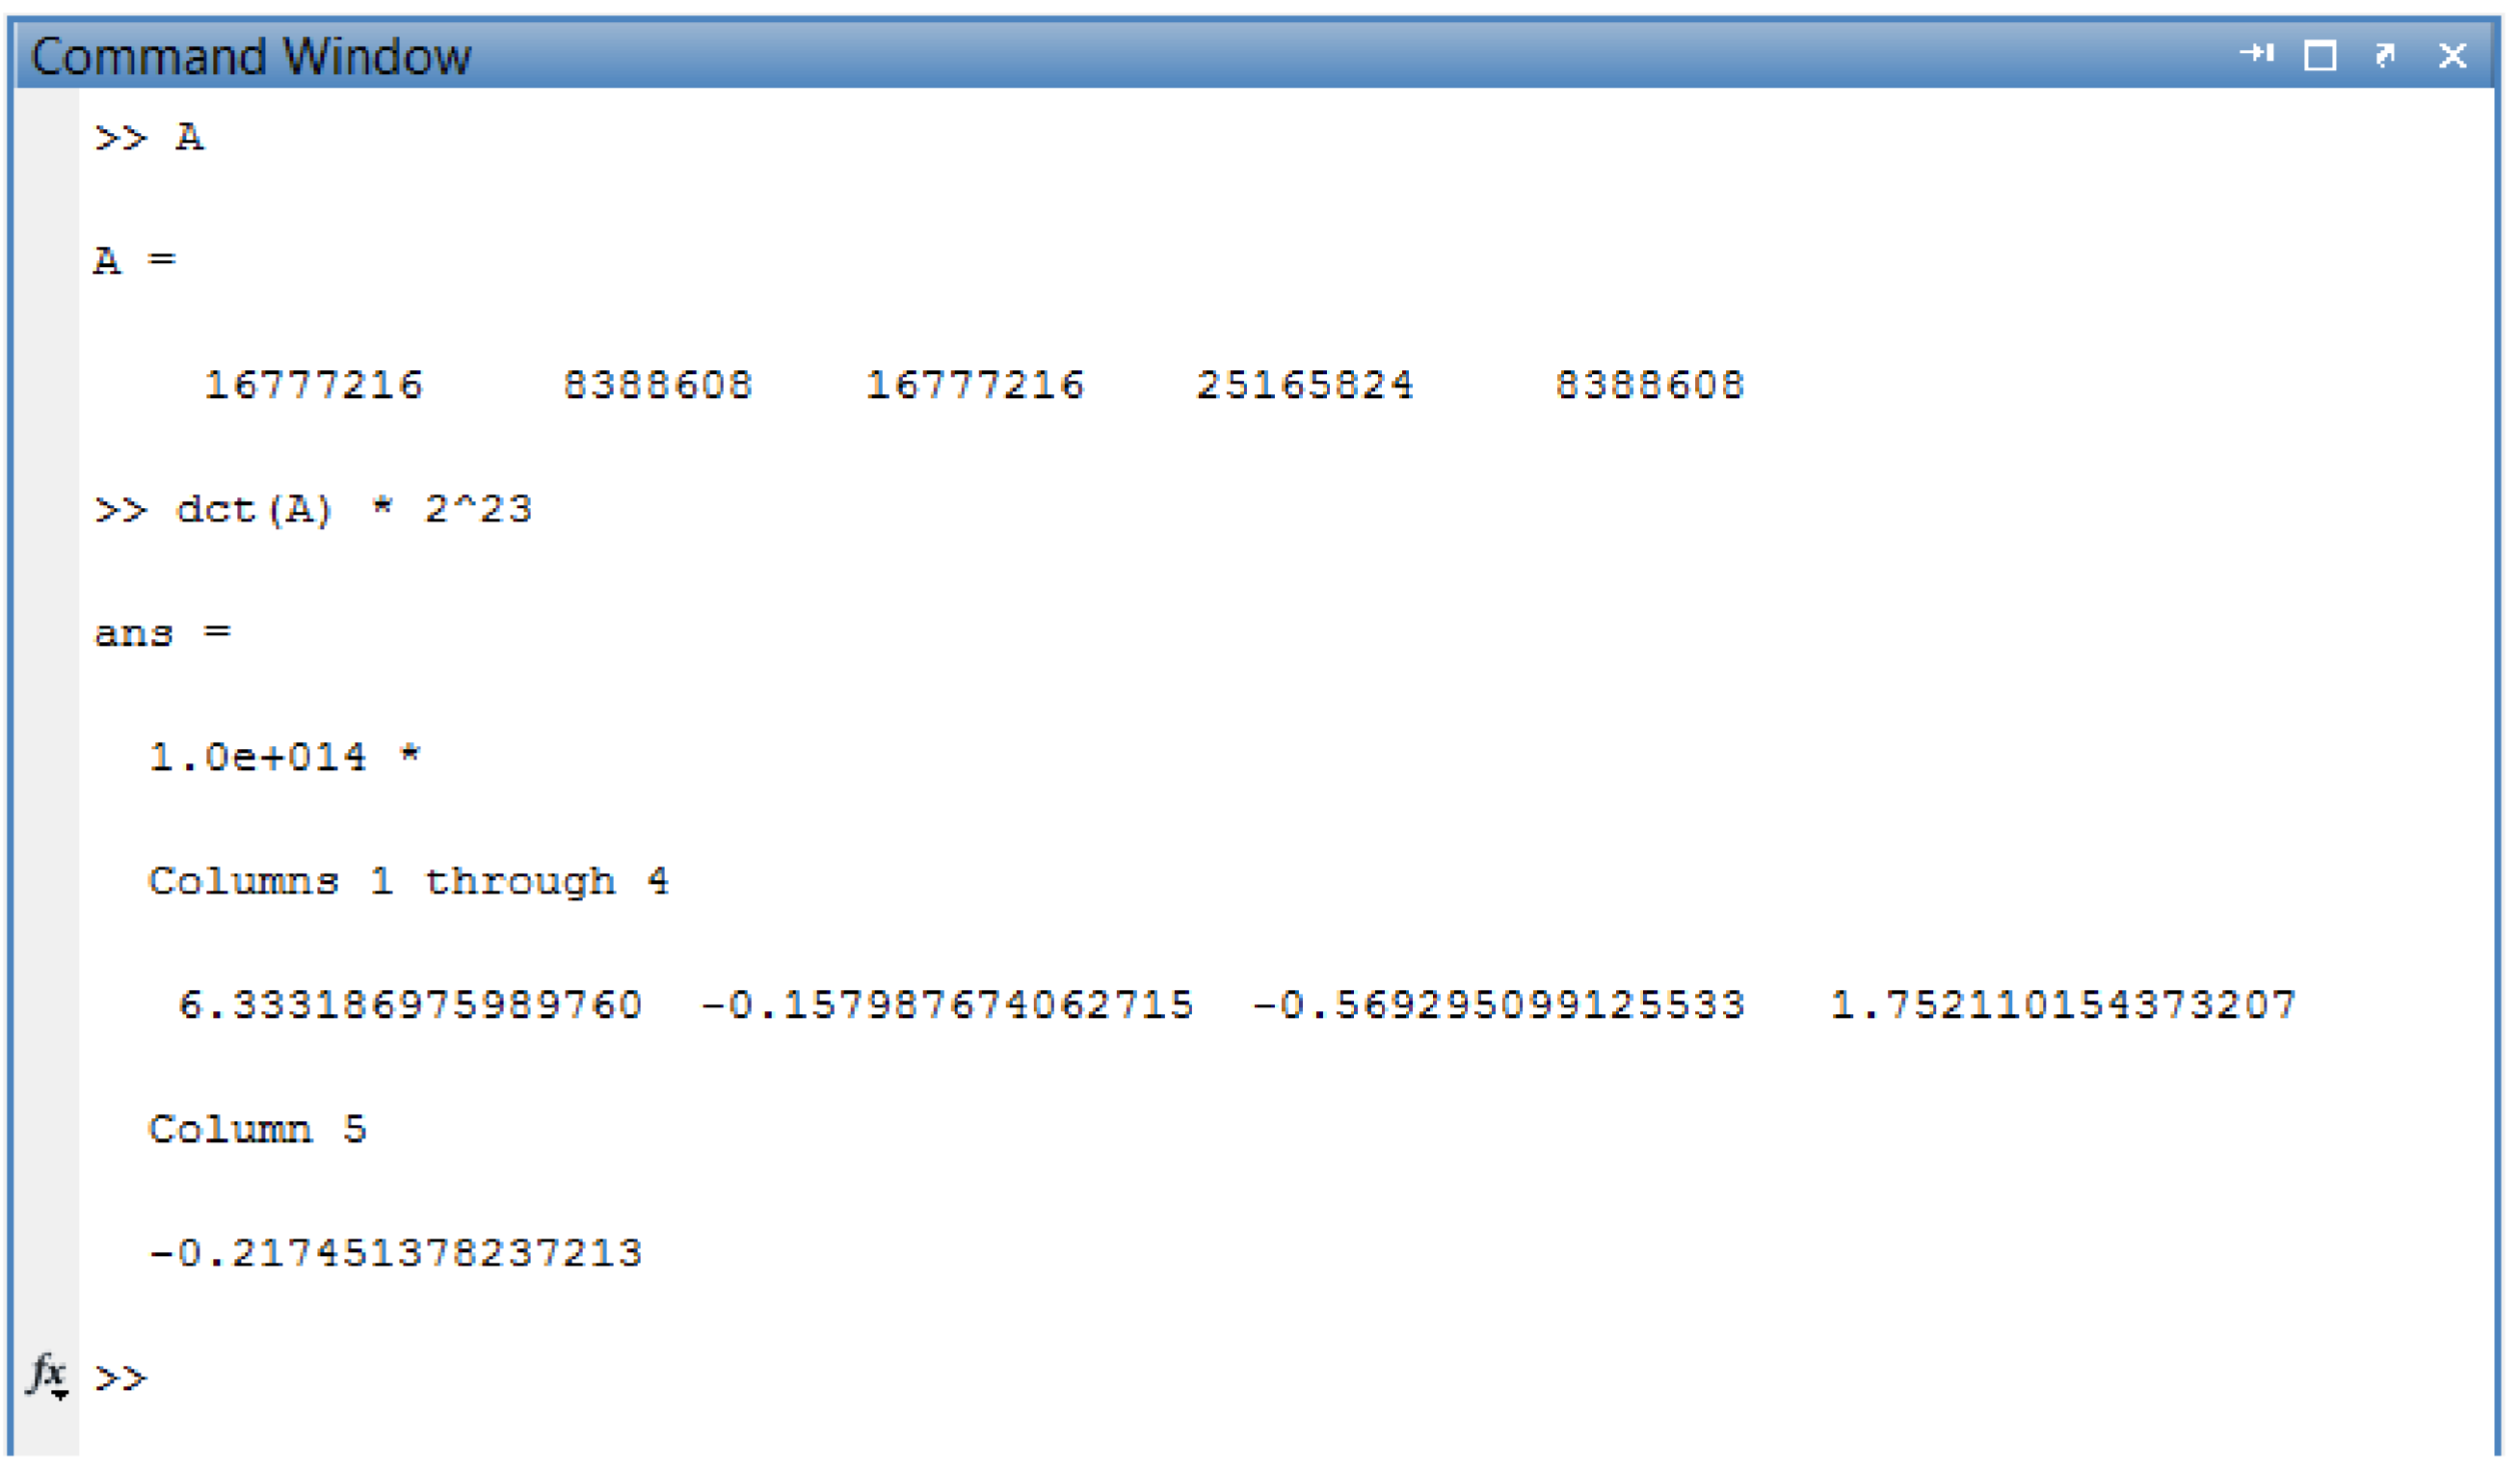
\includegraphics[width=\textwidth]{imm/dct/dct_sa4.png}  
        	\caption{Check results in MATLAB for systolic array architecture} 
        	\label{fig:dct_sa4}
        \end{figure}
   \clearpage
   \section{LLM DCT}
   There's a faster DCT algorithm, sometimes called LLM for its authors: Loeffler, Ligtenberg, and Moschytz.
   As said before (section \ref{DCT}), we use this formula for the computation of the Discrete Cosine Transformation.
   \bigskip
   
     \begin{equation} \label{eq:dct_eq_1}	
     X_{k}= \sum_{n=0}^{N-1} w(k)x_{n}cos\bigg[\frac{\pi}{N} (n+\frac{1}{2})k\bigg], \qquad k=0,1,...,N-1
     \end{equation}
     
     
     \[
     w(x)=\left\{
     \begin{array}{ll}
     \frac{1}{\sqrt{N}} & \qquad k=0\\
     &\\
     \sqrt{\frac{2}{N}} & \qquad 1\leqslant k \leqslant N-1\\
     \end{array}
     \right.
     \]
     \bigskip
     
     It has been found that for a certain kind of matrix, we can reduce the number of multiplications.\\
     In this work I present the algorithm for a 8-point DCT.\\
     First of all, let's have a look to the cosine matrix.
     Setting $ \gamma(k)=cos(\frac{2\pi k}{32}) $ the 8-point DCT matrix is
     \bigskip
     
     \begin{center}	
     	$ \dfrac{1}{2}\begin{bmatrix} \gamma(4)  & \gamma(4) &\gamma(4)  & \gamma(4) &\gamma(4)  & \gamma(4) &\gamma(4)  & \gamma(4) \\
     	
     	\gamma(1)  & \gamma(3) &\gamma(5)  & \gamma(7) &-\gamma(7)\qquad  & -\gamma(5)\qquad &-\gamma(3) \qquad & -\gamma(1) \qquad      	\\
     	
    \gamma(2)  & \gamma(6) &-\gamma(6) \qquad & -\gamma(2) \qquad&-\gamma(2)  & -\gamma(6) &\gamma(6)  & \gamma(2)\\ 

\gamma(3)  & -\gamma(7) &-\gamma(1)  & -\gamma(5) &\gamma(5)  & \gamma(1) &\gamma(7)  & -\gamma(3)\\
 
\gamma(4)  & -\gamma(4) &-\gamma(4)  & \gamma(4) &\gamma(4)  & -\gamma(4) &-\gamma(4)  & \gamma(4)\\

\gamma(5)  & -\gamma(1) &\gamma(7)  & \gamma(3) &-\gamma(3)  & -\gamma(7) &\gamma(1)  & -\gamma(5)\\
     
\gamma(6)  & -\gamma(2) &\gamma(2)  & -\gamma(6) &-\gamma(6)  & \gamma(2) &-\gamma(2)  & \gamma(6)\\

\gamma(7) \qquad & -\gamma(5) \qquad&\gamma(3)  & -\gamma(1) &\gamma(1)  & -\gamma(3) &\gamma(5)  & -\gamma(7)\\   
      \end{bmatrix} $
     	
     \end{center}
     \bigskip
     We know that the DCT can be seen as a product of matrices:
     
     	\begin{center}
     		\bigskip	
     		$\begin{bmatrix}X_{0}\\ X_{1} \\ X_{2}\\X_{3}\\ X_{4} \\ X_{5} \\X_{6} \\X_{7} \end{bmatrix} = 
     		\dfrac{1}{2}\begin{bmatrix} \gamma(4)  & \gamma(4) &\gamma(4)  & \gamma(4) &\gamma(4)  & \gamma(4) &\gamma(4)  & \gamma(4) \\
     		
     		\gamma(1)  & \gamma(3) &\gamma(5)  & \gamma(7) &-\gamma(7)\qquad  & -\gamma(5)\qquad &-\gamma(3) \qquad & -\gamma(1) \qquad      	\\
     		
     		\gamma(2)  & \gamma(6) &-\gamma(6) \qquad & -\gamma(2) \qquad&-\gamma(2)  & -\gamma(6) &\gamma(6)  & \gamma(2)\\ 
     		
     		\gamma(3)  & -\gamma(7) &-\gamma(1)  & -\gamma(5) &\gamma(5)  & \gamma(1) &\gamma(7)  & -\gamma(3)\\
     		
     		\gamma(4)  & -\gamma(4) &-\gamma(4)  & \gamma(4) &\gamma(4)  & -\gamma(4) &-\gamma(4)  & \gamma(4)\\
     		
     		\gamma(5)  & -\gamma(1) &\gamma(7)  & \gamma(3) &-\gamma(3)  & -\gamma(7) &\gamma(1)  & -\gamma(5)\\
     		
     		\gamma(6)  & -\gamma(2) &\gamma(2)  & -\gamma(6) &-\gamma(6)  & \gamma(2) &-\gamma(2)  & \gamma(6)\\
     		
     		\gamma(7) \qquad & -\gamma(5) \qquad&\gamma(3)  & -\gamma(1) &\gamma(1)  & -\gamma(3) &\gamma(5)  & -\gamma(7)\\   
     		\end{bmatrix} \begin{bmatrix}x_{0}\\ x_{1} \\ x_{2}\\x_{3}\\ x_{4} \\ x_{5} \\x_{6} \\x_{7} \end{bmatrix}$
     		
     	\end{center}
     	\bigskip
 More explicitly
 \begin{flushleft}
 \qquad	\quad$ X_{0}= (x_{0}+ x_{1} +x_{2}+x_{3}+ x_{4} + x_{5} +x_{6} +x_{7})\cdot \gamma(4)$\\
 \qquad	\quad	$  X_{1}=(x_{0}-x_{7})\cdot \gamma(1)+(x_{1}-x_{6})\cdot \gamma(3)+(x_{2}-x_{5})\cdot \gamma(5)+(x_{3}-x_{4})\cdot \gamma(7)$\\
 \qquad	\quad	$  X_{2}=[(x_{0}+x_{7})-(x_{3}+ x_{4})]\cdot \gamma(2)+ [(x_{1}+x_{6})-(x_{2}+x_{5})]\cdot \gamma(6)$\\
 \qquad	\quad	$   X_{3}=(x_{0}-x_{7})\cdot \gamma(3)+(x_{6}-x_{1})\cdot \gamma(7)+(x_{5}-x_{2})\cdot \gamma(1)+(x_{4}-x_{3})\cdot \gamma(5)$\\
 \qquad	\quad	$  X_{4}=(x_{0}+ x_{7} +x_{3}+ x_{4})\cdot \gamma(4)-( x_{5} +x_{6} +x_{1}+x_{2})\cdot\ \gamma(4)$\\
 \qquad	\quad	$  X_{5}=(x_{0}-x_{7})\cdot \gamma(5)+(x_{6}-x_{1})\cdot \gamma(1)+(x_{2}-x_{5})\cdot \gamma(7)+(x_{3}-x_{4})\cdot \gamma(3)$\\
 \qquad	\quad	$  X_{6}=[(x_{0}+x_{7})-(x_{3}+ x_{4})]\cdot \gamma(6)+ [(x_{2}+x_{5})-(x_{1}+x_{6})]\cdot \gamma(2)$\\
 \qquad	\quad	$  X_{7}=(x_{0}-x_{7})\cdot \gamma(7)+(x_{6}-x_{1})\cdot \gamma(5)+(x_{2}-x_{5})\cdot \gamma(3)+(x_{4}-x_{3})\cdot \gamma(1)$\\
 \end{flushleft}
 \bigskip
 we can see that we can do some addition in parallel and some of them in series due to the data dependencies.\\
 Moreover, we can reduce the number of multiplications. For instance for $ X_{0} $ we need only one multiplication, and for $ X_{4} $ only 2.
 \subsection{Architecture of the LLM DCT} \label{llmarch}
 The architecture is shown in fig \ref{dct8}
        \begin{figure}[h!]
        	\centering
        	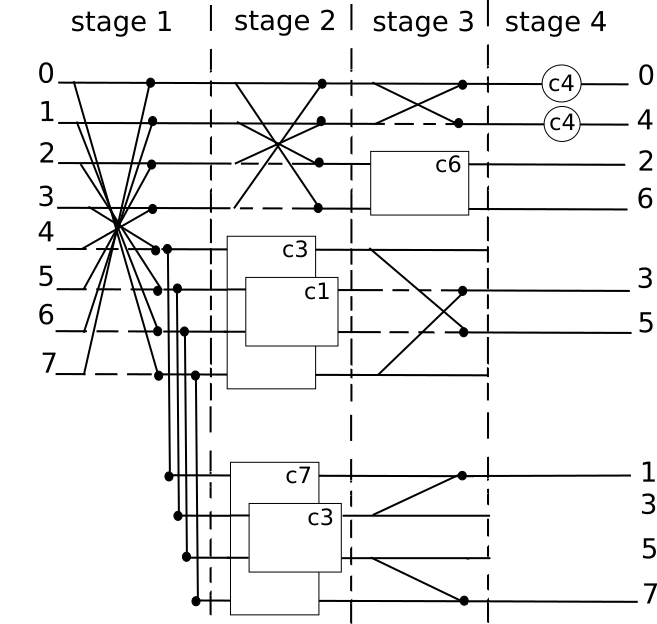
\includegraphics[width=\textwidth]{imm/dct/dct8.png} 	\caption{LLM DCT for an 8-point with 17 multiplications. For symbols, see figure \ref{dct8_scheme}} 
        	\label{dct8}
        \end{figure}

        The stages of the LLM Algorithm for an 8-point DCT, numbered 1 to 4, are parts that have to be executed in series and can not be evaluated in parallel because of data dependencies. However calculations inside one stage can be parallelized. \\
        Stage 1 consists of 8 additions/subtractions. \\
        In Stage 2 , the algorithm splits into two parts. One part is for even coefficients (only additions and subtractions) and the second part is for odd coefficients (rotations). \\
         The even part is nothing else than a 4-point DCT, again separating in even and odd part in stage 3.\\
         Figure \ref{dct8_scheme} explains the building blocks of the algorithm.  
     The second building block, the rotation, can be calculated using only 3 multiplications and 3 additions instead of 4 multiplications and 2 additions using the equivalence shown in equation \ref{rot_eq}.
     Since $ a=cos(\frac{n\pi}{2N}) $ and $ b=sin(\frac{n\pi}{2N}) $ are constants and known \textit{a priori}, also the values $ (b-a) $ and $ -(b+a) $ are constants, so we do not need an hardware component to compute them.
     \begin{equation}\label{rot_eq}
     \begin{aligned}
     	y_{0}\quad=&a\cdot x_{0} + b\cdot x_{1} \quad=& (b - a)\cdot x_{l}+a\cdot (x_{0}+x_{l})\\
     	y_{0}= & -b\cdot x_{0} + a\cdot x_{1}= &  -(b+a)\cdot x_{0}+a\cdot (x_{0}+x_{l})\\
     	a=&cos(\frac{n\pi}{2N})&\\
     	b=&sin(\frac{n\pi}{2N})&
     	\end{aligned}
     \end{equation}
     \bigskip
              \begin{figure}[h!]
              	\centering
              	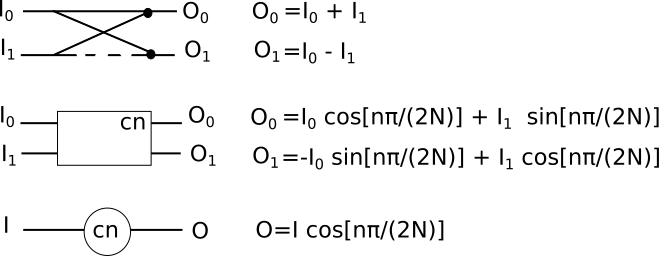
\includegraphics[width=\textwidth]{imm/dct/dct8_scheme.png} 	\caption{Symbols used to describe the LLM DCT for an 8-point with 17 multiplications (fig.\ref{dct8})} 
              	\label{dct8_scheme}
              \end{figure}
        
        
       
    \subsection{Simulation and test}
    I performed some tests of this implementation with different values. \\In the fig.\ref{tb_dct8} we can see the results of an array of 8 elements using the LLM structure.\\
    \bigskip
  \begin{figure}[h!]
              	\centering
              	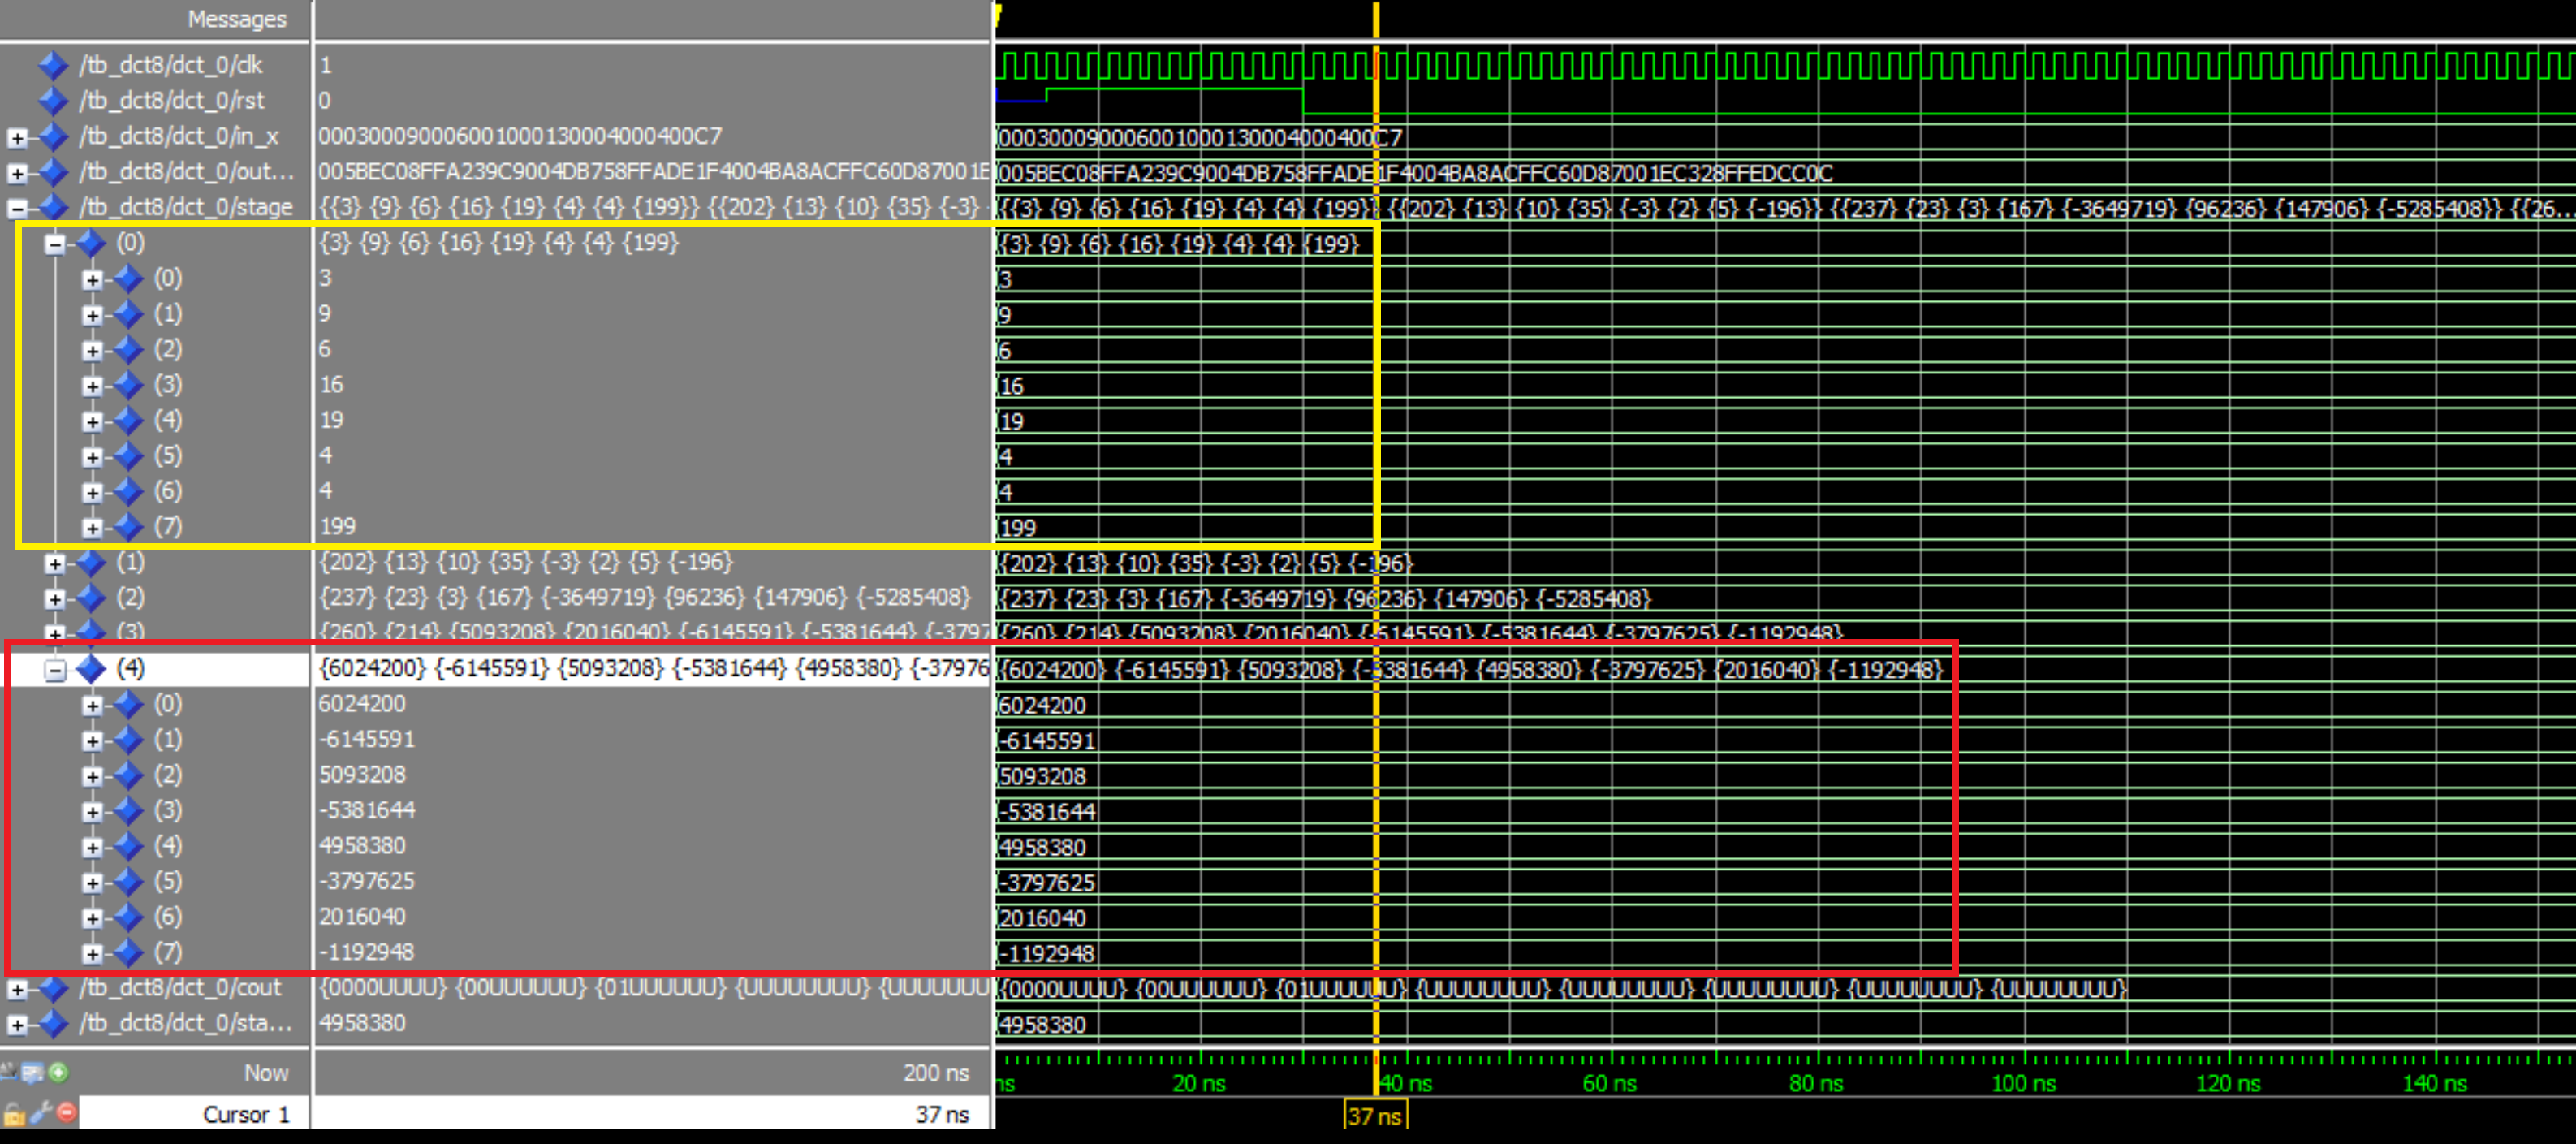
\includegraphics[width=\textwidth]{imm/dct/tb_dct8.png} 	\caption{LLM 8-point Discrete cosine transform-Results of the simulation} 
              	\label{tb_dct8}
  \end{figure}
  \bigskip
  In the yellow box, we can see the input vector to be
  \begin{center}
  		$ x_{0}=3$\\
  		$ 	x_{1}=9 $\\
  		$ x_{2}=6 $ \\
  		$ x_{3}=16 $ \\
  		$ x_{4}=19 $ \\
  		$x_{5}=4$\\
  			$x_{6}=4$\\
  				$x_{7}=199$\\
  \end{center}
  Between the yellow box and the red box, we can see the results of the different stages.\\
  The final result is shown in the red box. Since we reserved 16 bits for the decimal part, these vector has to be shifted by 16 position, i.e. divided by $ 2^{16}=65536 $.
  
    \begin{center}
    	$ X_{0}=6024200/2^{16}=91.9219$\\
    	$ X_{1}=-6145591/2^{16}=-93.7742 $\\
    	$ X_{2}=5093208/2^{16}= 77.7161$ \\
    	$ X_{3}=-5381644/2^{16}= -82.1173$ \\
    	$ X_{4}=4958380/2^{16}= 75.65887$ \\
    	$X_{5}=-3797625/2^{16}=-57.9471$\\
    	$X_{6}=2016040/2^{16}=30.7623$\\
    	$X_{7}=-1192948/2^{16}=-18.2029$\\
    \end{center}
     We checked this result by using the function $ dct $ on Matlab (Figure \ref{fig:dct8_res_mat}).
     We see that it differs from the Matlab result by a value in the order of 1/100. This depends on the precision used for the implementation, especially when converting the cosine values into binary.
     
     
     
     
     
     \begin{figure}[h!]
     	\centering	
     	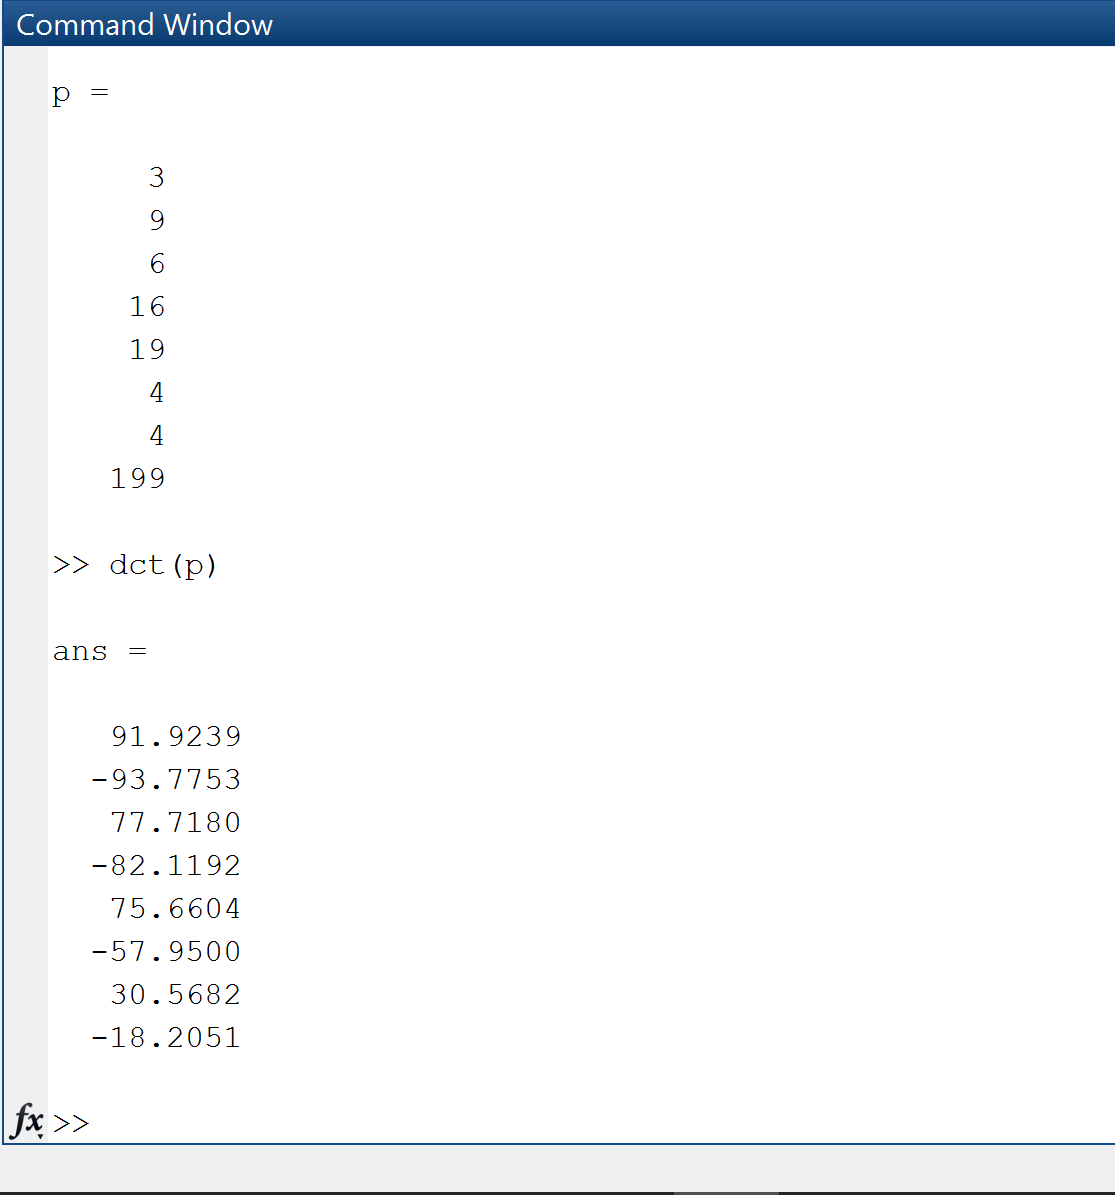
\includegraphics[width=0.9\textwidth]{imm/dct/dct8_matlab.png}  
     	\caption{LLM 8-point DCT result in MATLAB} 
     	\label{fig:dct8_res_mat}
     \end{figure}
     
     \subsection{Comparison}
     Since this architecture is fon an 8-point DCT, I will compare it with the other structure for the DCT shown before (subsection \ref{DCTH} and \ref{DCTSA}).
     \begin{center}
     	\begin{tabular}{ | p{1cm} |  p{2.5cm} |  p{2.5cm} | p{2.5cm} | p{2.5cm}|p{2.5cm}|}
     	\hline
     	\label{table:dct8_tab}N=8 & Systolic array & This work & This work pipelined & LLM & LLM pipelined\\
     	\hline
     	Area & $ 8^{2}$ \textit{multiplications} $8^{2}$ \textit{additions}&$8^{2}$ \textit{ moltiplications}  $ 8^{2}$\textit{additions} & $8$ \textit{moltiplications} $8$\textit{additions} & $17$ \textit{moltiplications} $33$\textit{additions} & $4.25
     	$ \textit{moltiplications}  $ 8.25$\textit{additions}\\ 
     	\hline
     	Time &$(2\cdot8-1)$ x \textit{(time for a multiplication followed by an addition)}&
     	$ 8 $ x \textit{(time for a multiplication followed by an addition)}&\textit{time for a multiplication followed by an addition}&\textit{time for 3 multiplications and 6 addition}&\textit{time for 1 multiplication and 2 additions}\\      	
     	\hline     
     		
     	\end{tabular}
     \end{center}
     \bigskip
     We can see that the LLM (both pipelined and not) is the best solutions in terms of area.\\
     In terms of time, if we look to the pipelined LLM architecture, we have to consider the longest critical path between the four stages. This is found in the rotation block, which takes the time for a multiplication and 2 additions. The Data Flow Graph is shown in fig. \ref{rot}.
          \begin{figure}[h!]
          	\centering	
          	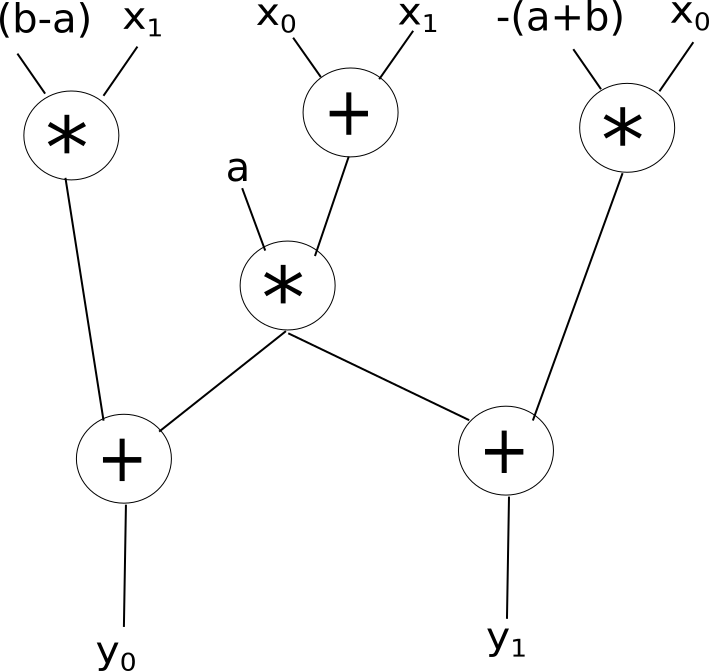
\includegraphics[width=0.7\textwidth]{imm/dct/rot.png}  
          	\caption{DFG for a rotation block} 
          	\label{rot}
          \end{figure}
     So looking to the pipelined architectures of the LLM and the one shown in this work (subsection \ref{DCTH}), it's better the one i presented above.\\
     If we look to the architecture without any pipeline register, the critical path will be 1 multiplication and 4 additions. To find this value, we can consider the critical path for each output element, by taking into account that a rotation block take the time for one multiplication and 2 additions.
     A scheme is shown in fig. \ref{dfg_llm}.
               \begin{figure}[h!]
               	\centering	
               	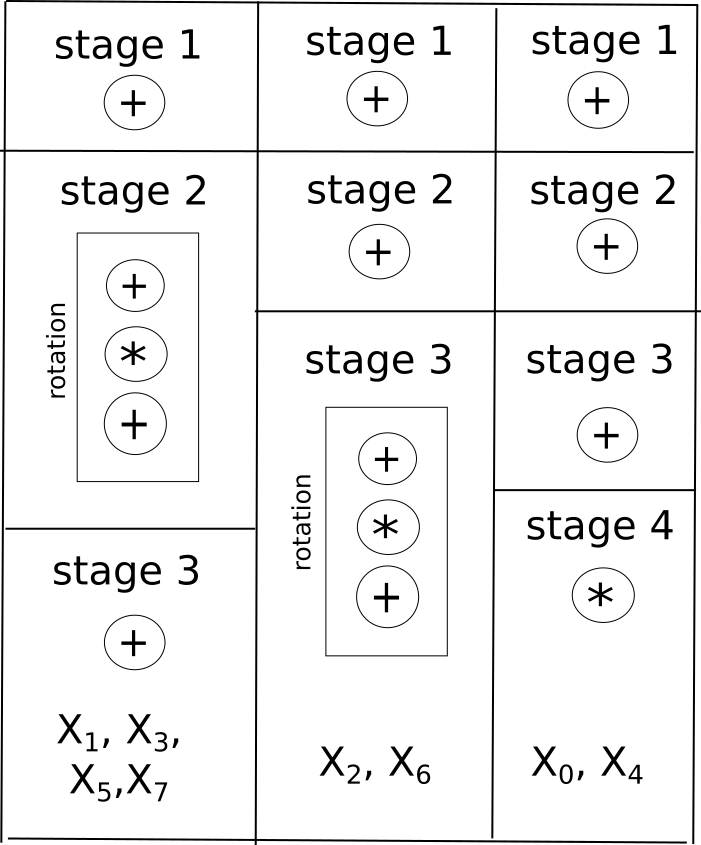
\includegraphics[width=\textwidth]{imm/dct/dfg_llm.png}  
               	\caption{Critical path for each output element} 
               	\label{dfg_llm}
               \end{figure}
      In conclusion, without any pipeline registers, it's better the LLM architecture in terms of time.
 
          \clearpage        
          \newpage
          \subsection{High Order LLM DCT} \label{HLLM}
          Many studies has been done for the LLM architecture, and it has been theorized that the LLM can be applied for the DCT that has a size of $ 2^{n}$.\\
 Although we can see a recursive approach for the even parts at top, such as an addition/substraction, nothing can be said for the odd parts. A brute-force search is required.\\
 Fig. \ref{dct16} and fig. \ref{dct32} show an implementation for the LLM of order-16 and order-32 respectively.  
\begin{figure}[h!]
     	\centering	
     	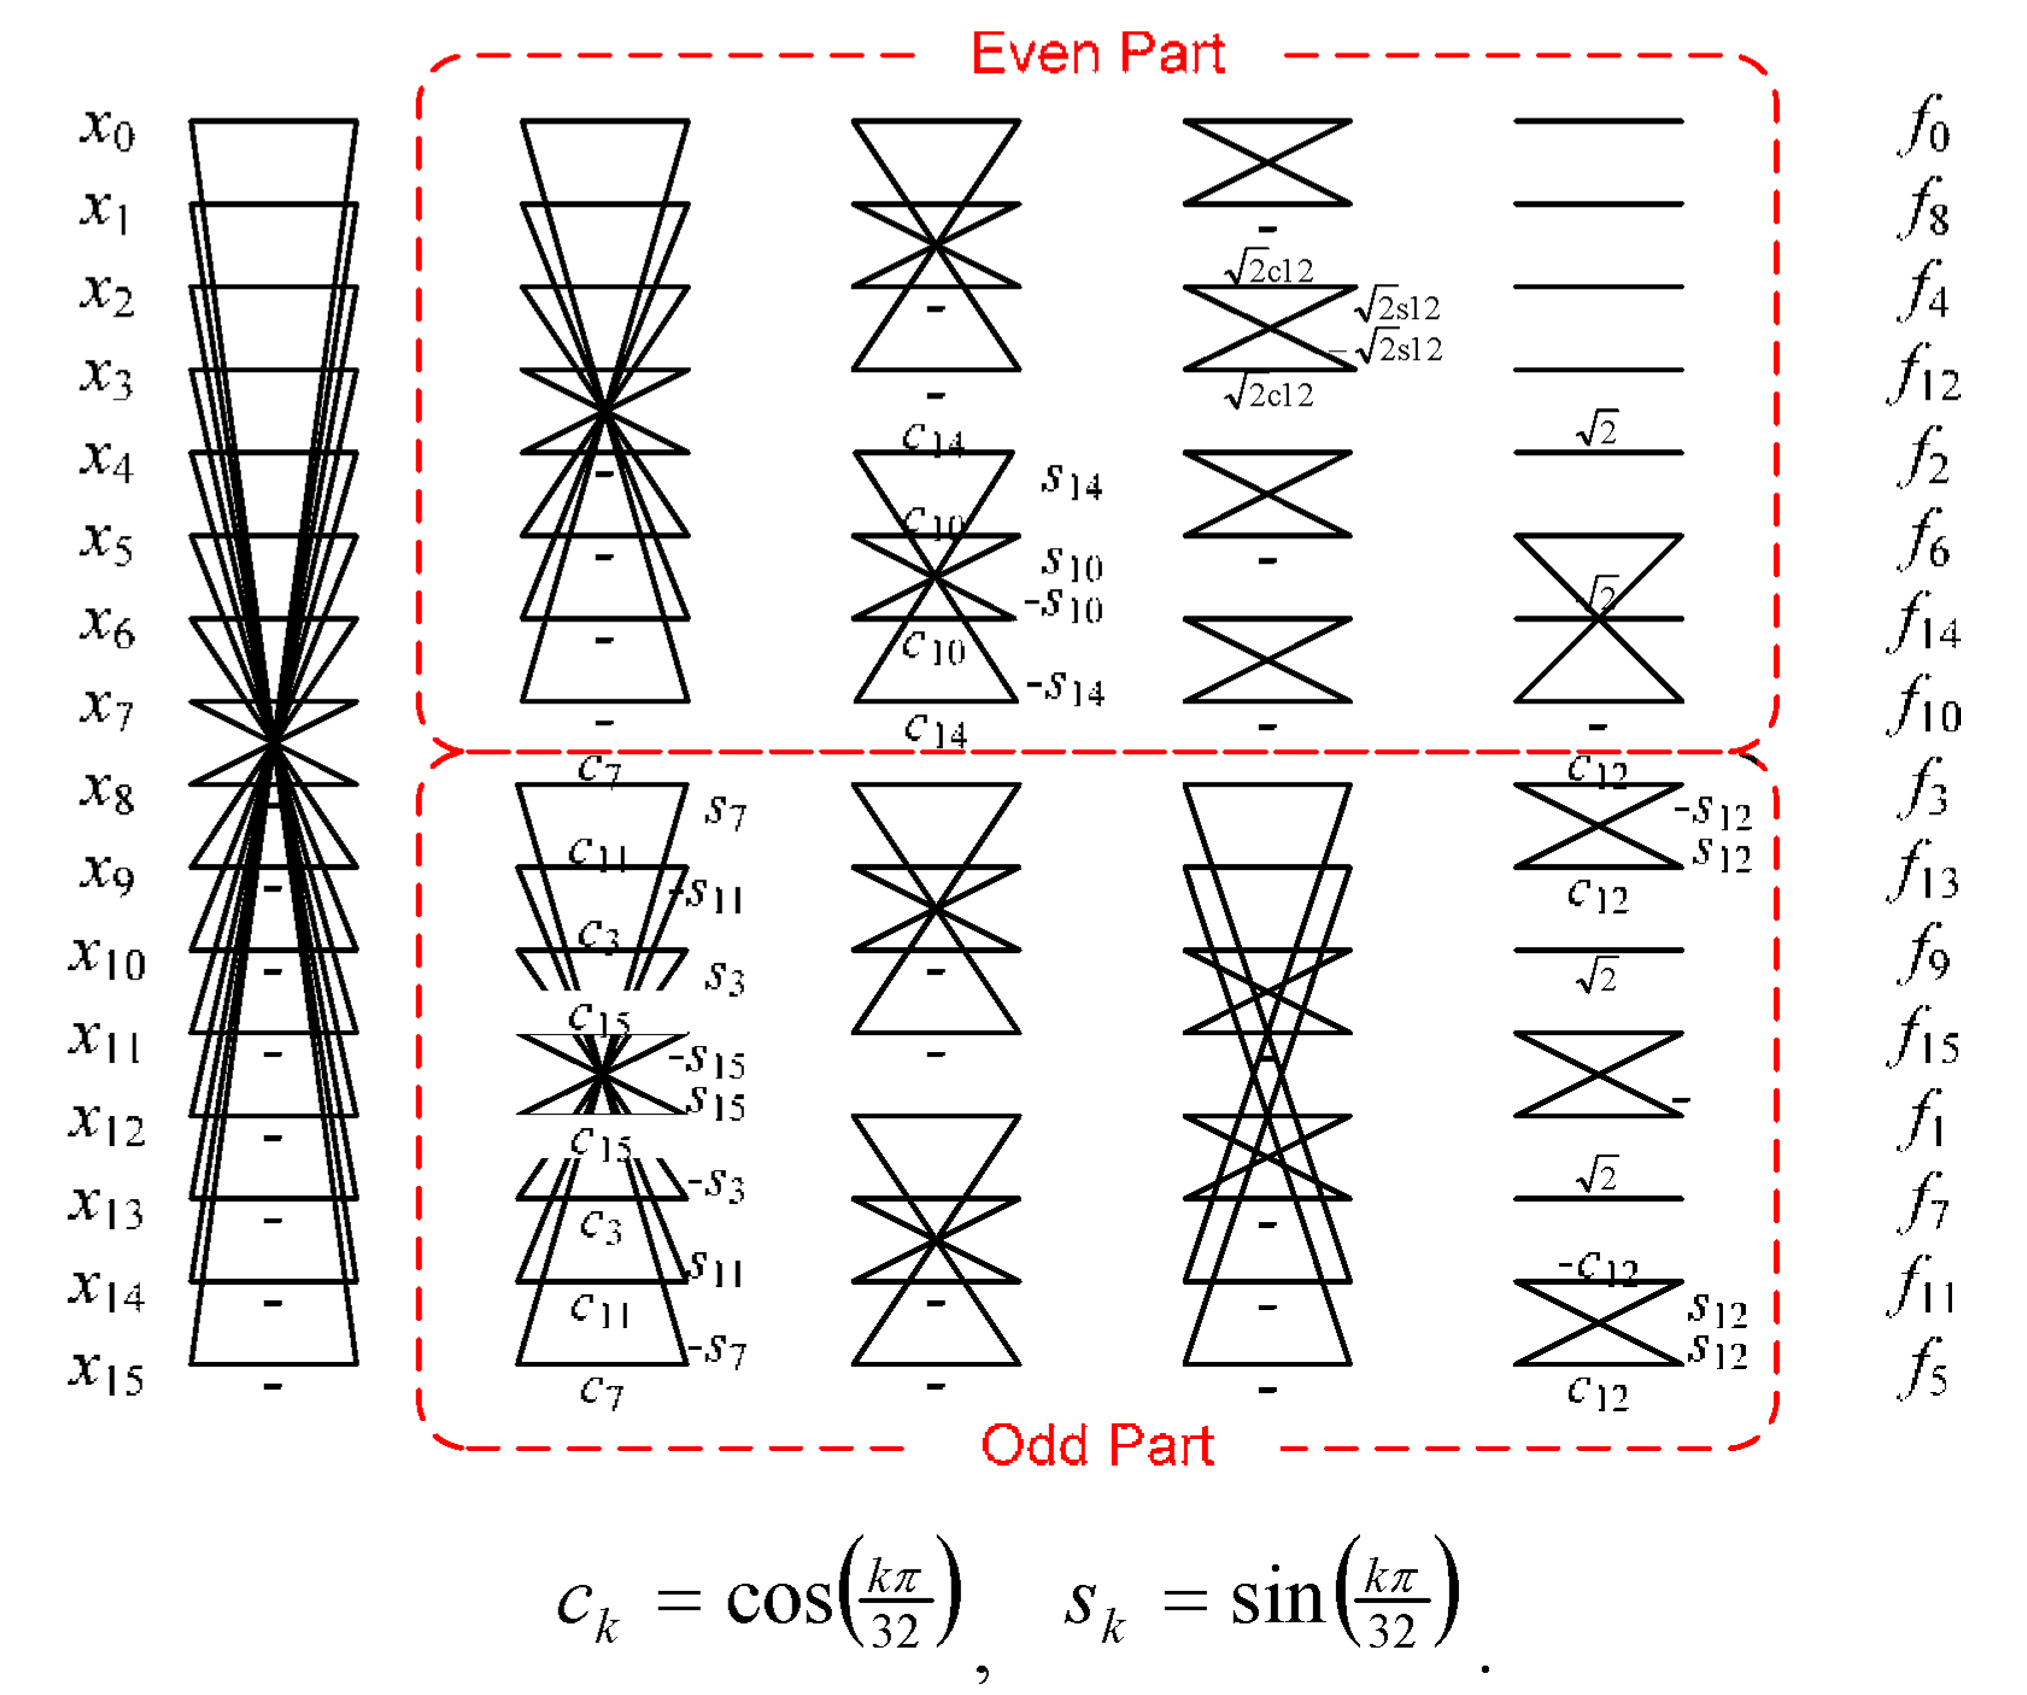
\includegraphics[width=\textwidth]{imm/dct/dct16.png}  
     	\caption{Order-16 LLM fast DCT algorithm} 
     	\label{dct16}
\end{figure} 

\begin{figure}[h!]
     	\centering	
     	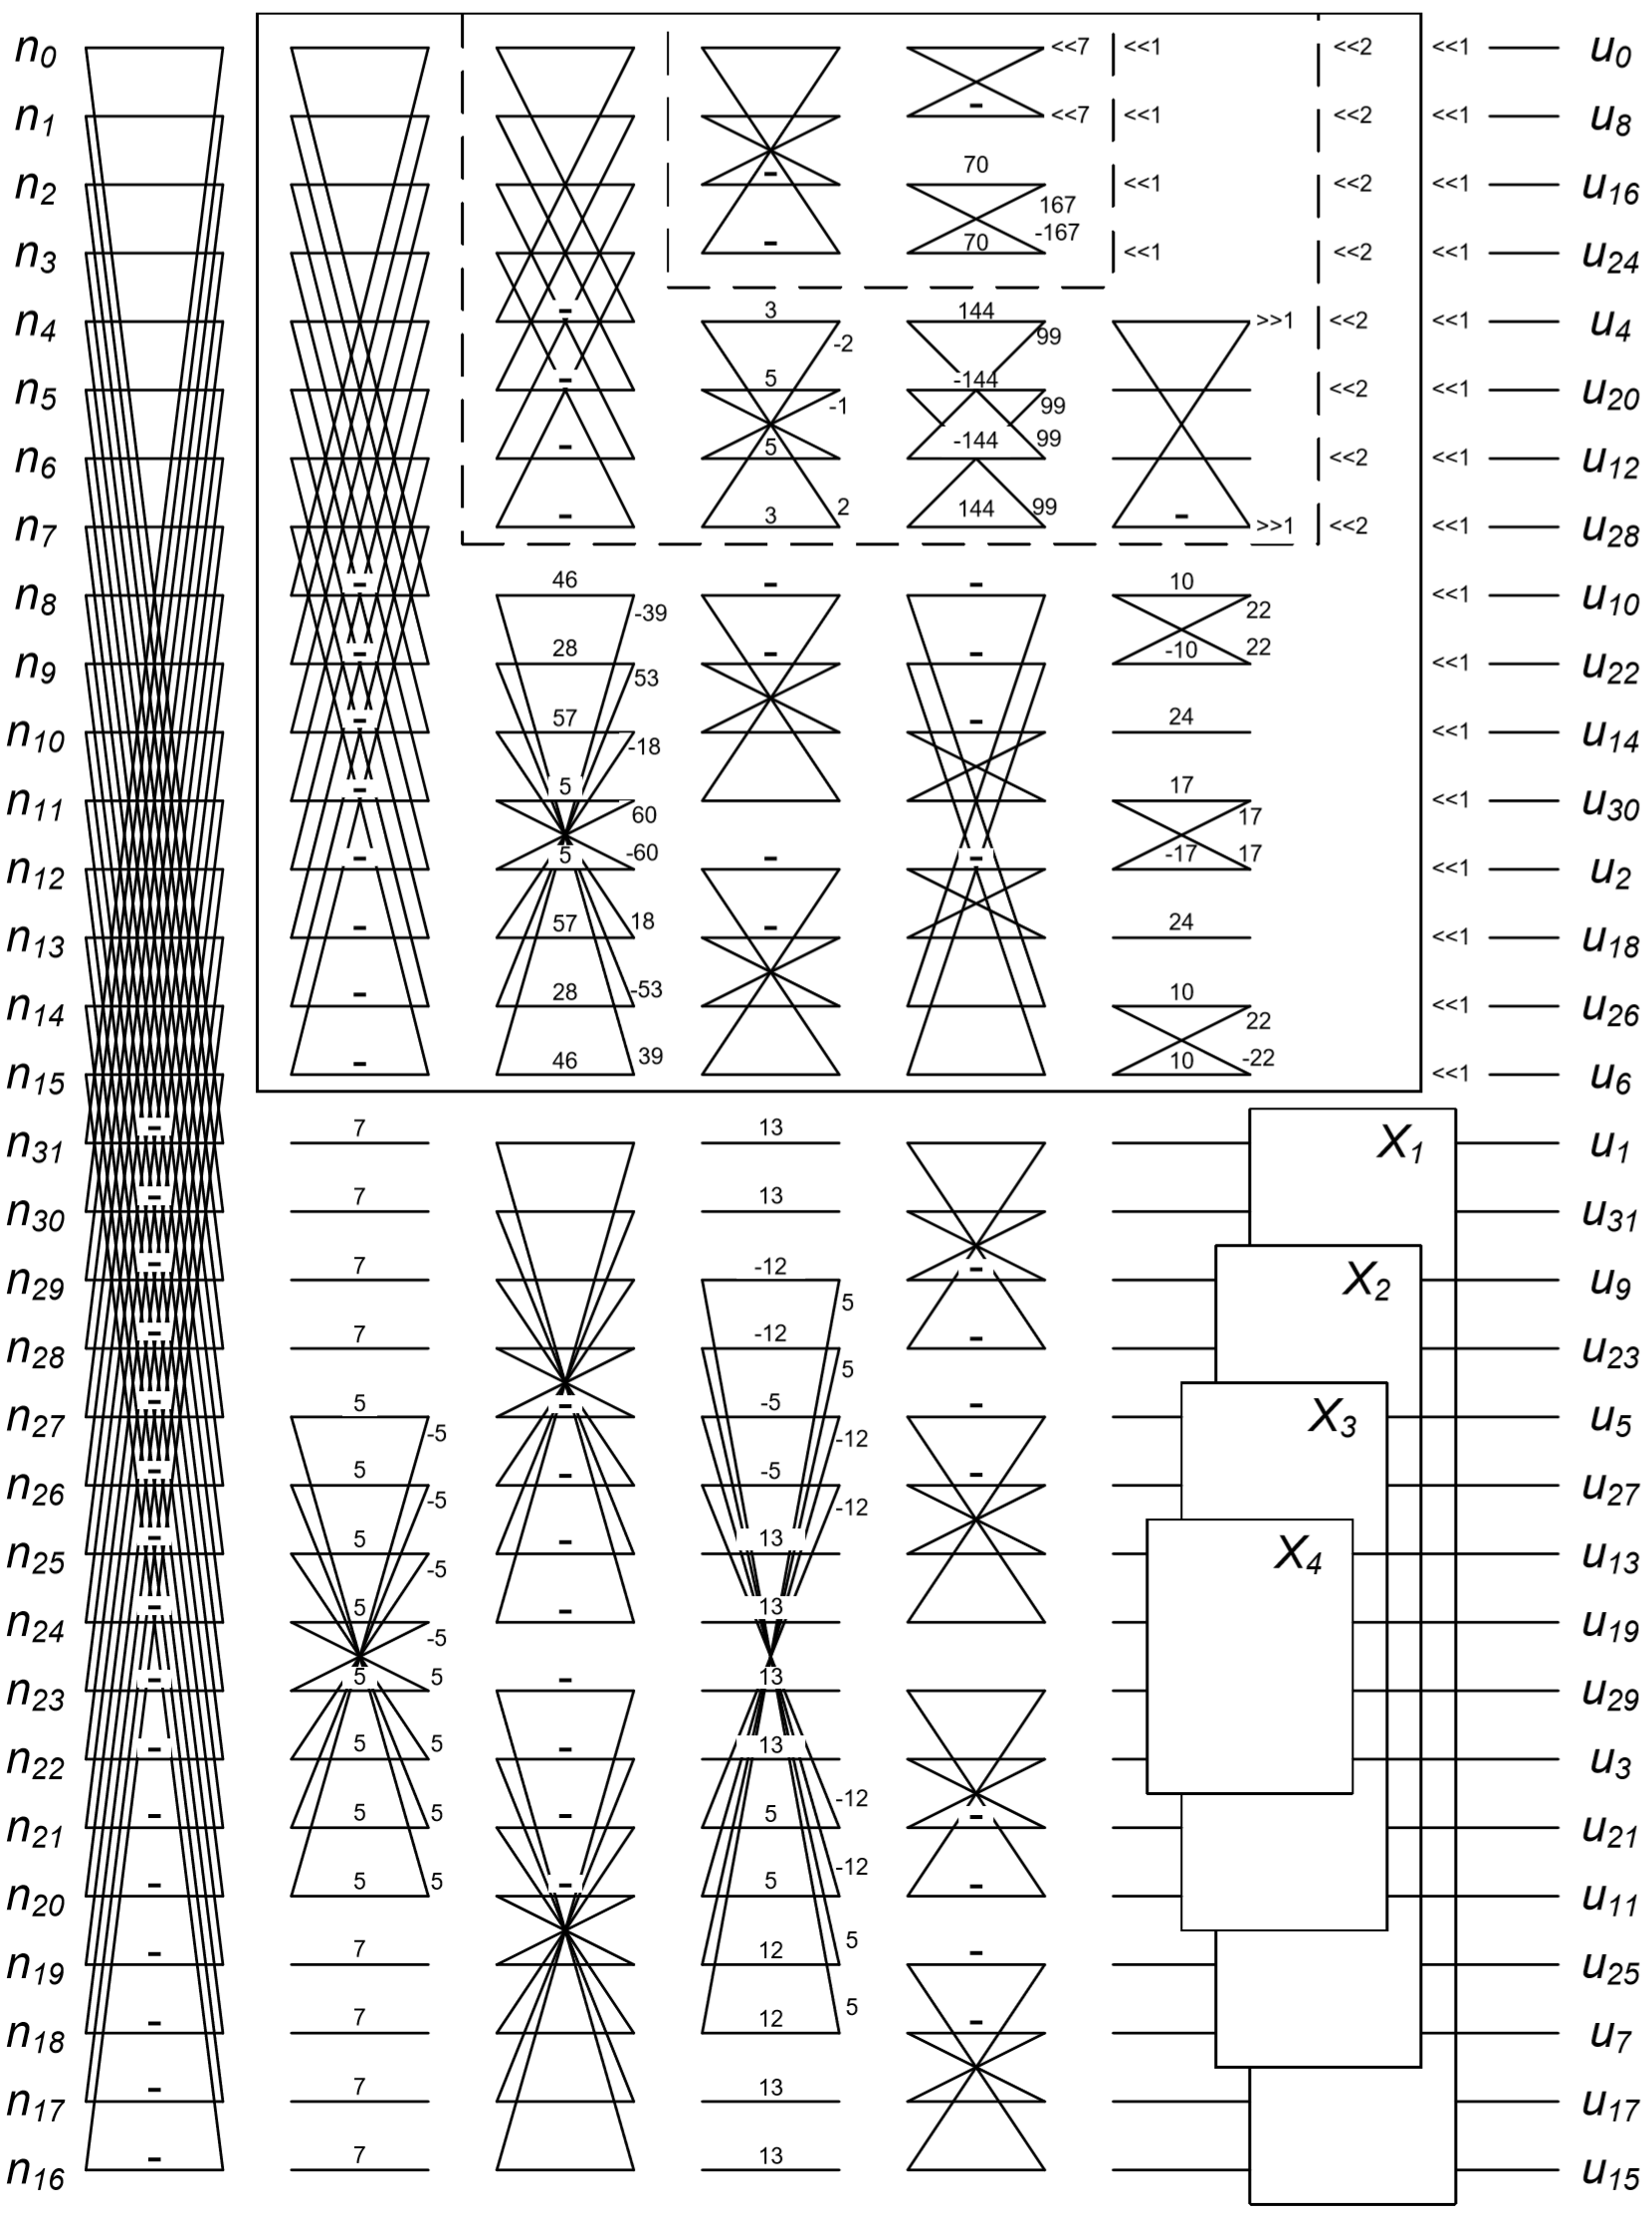
\includegraphics[width=\textwidth]{imm/dct/dct_2n.png}  
     	\caption{ Fast algorithm for the forward order-32 integer transform with the fast algorithms for the forward order-4, order-8, and order-16 integer transforms embedded. } 
     	\label{dct32}
\end{figure}  

        
